\documentclass[11pt]{article}

\usepackage[utf8]{inputenc}
%%\usepackage[T1]{fontenc}
\usepackage{graphicx}
\usepackage[linktocpage=true]{hyperref}

%%Page layout
\usepackage[margin=2.0cm]{geometry}
\usepackage{bookmark}

%%Table Colours
\usepackage{color}
\definecolor{blue}{rgb}{0.392,0.584,0.929}
\usepackage{colortbl}

%%For Use Case Scenarios
\usepackage{eulervm}
\usepackage[charter]{mathdesign}
\usepackage{xcolor}

%%Figures
\usepackage{float}

\usepackage{mathpazo}

%%Font and Numbers
\renewcommand*\rmdefault{dayrom}
\usepackage[T1]{fontenc}
\normalfont
\usepackage{enumitem}

%%Packages for Referrences
\usepackage{url}
\usepackage{etoolbox}
\patchcmd{\thebibliography}{\section*{\refname}}{}{}{}
\patchcmd{\thebibliography}{\addcontentsline{toc}{section}{\refname}}{}{}{}

%%Group Comments
\usepackage{verbatim}

\usepackage{titlesec}

\setcounter{secnumdepth}{4}

\titleformat{\paragraph}
{\normalfont\normalsize\bfseries}{\theparagraph}{1em}{}
\titlespacing*{\paragraph}
{0pt}{3.25ex plus 1ex minus .2ex}{1.5ex plus .2ex}

\begin{document}
\renewcommand{\familydefault}{\sfdefault}
\begin{titlepage}
	\newcommand{\HRule}{\rule{\linewidth}{0.5mm}}
	\begin{center}
		            
		\textsc{\LARGE Alabama Liquid Snake}\\[0.8cm]
		\textsc{\Large University of Pretoria}\\[0.5cm]
		\textsc{\large Epi-Use}\\[0.5cm]
		    
		\HRule\\[0.4cm]
		    	
		{\huge\bfseries Botic - Privacy aware chatbot}\\[0.2cm]
		    	
		{\huge Process and Methodology}\\[0.2cm]
		
		\HRule\\[0.5cm]
		
		\textsc{Justin Grenfell} - u16028440 \\[0cm]
		\textsc{Peter Msimanga} - u13042352 \\[0cm]
		\textsc{Alicia Mulder} - u14283124 \\[0cm]
		\textsc{Kyle Gaunt} - u15330967 \\[0cm]
		\textsc{Lesego Mabe} - u15055214 \\[0cm]
		    
	\end{center}
\end{titlepage}
\tableofcontents
\newpage

\section{Introduction}
\subsection{Agile Unified Methodology}

%<Provide a Diagram of the AUM>

Using the Agile Unified Methodology to take advantage of agile principles as well as work with a methodology based off the
waterfall process, that has a simple linear and uncomplicated progression is what we have chosen to do. We anticipate that
the project will not have a high requirements change throughout development, and this makes the waterfall process derivative
methodology more fitting.

The Agile Unified Methodology makes use of Test-Driven Development, which makes it easier to develop high quality code.

%<Provide details of how we would deal with the set backs of the Test-Driven Development>
%<Additional motivations>

At the moment, phase 3 has high priority.

\section{Planning Phase}

\subsection{Acquiring Requirements}

\subsubsection{Specific Functional Requirements and Constraints}

\paragraph{User Interface}
\begin{itemize}
  \item[] R1.1 The system must allow a customer to enter a query and click on a button to send it.
  \item[] R1.2 The system must warn a customer of personal information included in a query.
  \item[] R2.2 The system must be able to highlight personally identifying information according to severity index.
  \item[] R3.3.2.2 The system must be able to highlight personally identifying information according to severity index.
  \item[] R3.3.2.3 The system must be able to warn the client representative if they have entered identifying information.
  \item[] R4.1 The system must allow customers to thumbs up a query response.
  \item[] R4.2 The system must allow customers to thumbs down a query response.
  \item[] R5 The system must allow queries to be sent to customer support representatives if not answered satisfactorily.
  \item[] C1 The system must use an Angular Single Page Application for the user interface.
\end{itemize}

\paragraph{Information Scraper}
\begin{itemize}
  \item[] R2.1 The system must be able to attach a severity to the personally identifying information.
  \item[] R3.1 The system must scrape its customer query responses for personal information.
  \item[] R3.3.2.1 The system must be able to identify personal information in a customer representative's response. 
  \item[] C3.1 The system must use word2vec for identifying personal information in customer queries.
  \item[] C5.2 The system must determine if the response contains personally identifying information.
\end{itemize}

\paragraph{Query Classification}
\begin{itemize}
  \item[] R3.2 The system must be able to classify the user queries.
  \item[] C3.2 The system must use word2vec for classifying customer queries.
\end{itemize}

\paragraph{Response Generation}
\begin{itemize}
  \item[] R3.3.1 The system must generate a response if it certain that it can.
  \item[] C5.1 The system must generate an automated response based on the query classification.
\end{itemize}

\paragraph{Chatbot}
\begin{itemize}
  \item[] R1.3 The system must be able to recieve customer queries.
  \item[] R3.3.2 The system must be able to send the query to a customer support representative if it cannot obtain an appropriate response.
  \item[] R3.4 The system must be able to send a query response back to a customer.
  \item[] R4.3 The system must be able to recieve customer feedback.
  \item[] R5 The system must allow queries to be sent to customer support representatives if not answered satisfactorily.
  \item[] R8 The system must interface with the currently existing ticket system.
  \item[] C2 The system must provide an API for the SPA to interact with.
\end{itemize}

\paragraph{Chatbot Trainer}
\begin{itemize}
  \item[] R6.1 The system must store previous customer interactions with positive feedback.
  \item[] R7 The system must must be trained with previous customer queries and responses.
  \item[] C4 The system must use Machine Learning or Deep Neural Networks in order to be trained with previous customer queries and responses.
\end{itemize}

\paragraph{Data Persistence}
\begin{itemize}
  \item[] R9.1 The system must scrape customer interation data for personal information before storing.
\end{itemize}

\subsubsection{Functional Clusters and Functional Subsystems}
\begin{center}
	\hspace*{-1.5cm}\begin{tabular}{|p{4cm}|p{7cm}|p{3cm}|p{5cm}|}
		\hline
		Functional Cluster & Functional Description & System Requirements & Function Subsystem Identified \\
		\hline
		User Interface & This functional cluster allows customers and customer support representatives to interact with the system & R1.1, R1.2, R2.2, R3.3.2.2, R3.3.2.3, R4.1, R4.2, R5, C1 & User Interface Subsystem \\
		\hline 
		Personal Information Identification & This functional cluster identifies personal information within messages & R2.1, R3.1, R3.3.2.1, C3.1, C5.2 & Message Scraper Subsystem \\
		\hline
		Classification of Queries & This functional cluster is responsible for classifying queries. & R3.2, C3.2 & Query Classification Subsystem \\
		\hline
		Automatic Query Response Generation & This functional cluster is responsible for generating query responses & R3.3.1, C5.1 & Response Generation Subsystem \\
		\hline
		Main Program & This function cluster is responsible for coordinating query handling subsystems & R1.3, R3.3.2, R3.4, R4.3, R5, R8, C2 & Chatbot Subsystem \\
		\hline
		ChatBot Training & This functional cluster is responsible for training the system using previous interactions & R6.1, R7, C4 & Chatbot Trainer Subsystem \\
		\hline
		 Data Persistence & This functional cluster is responsible for persisting customer interactions & R9.1 & Database Subsystem \\
		\hline
	\end{tabular}
\end{center}

\subsubsection{Traceability Matrix}
\begin{center}
	\hspace*{-1.3cm}\begin{tabular}{|c|c|c|c|c|c|c|c|}
	\hline
	R & UI & Info Scraper & Query Classification & Resp Generation & Chatbot & Chatbot Trainer & Data Persistence \\
	\hline
	R1.1 & X & & & & & & \\
	\hline
	R1.2 & X & & & & & & \\
	\hline
	R1.3 & & & & X & & & \\
	\hline
	R2.1 & & X & & & & & \\
	\hline
	R2.2 & X & & & & & & \\
	\hline
	R3.1 & & X & & & & & \\
	\hline
	R3.2 & & & X & & & & \\
	\hline
	R3.3.1 & & & & X & & & \\
	\hline
	R3.3.2 & & & & & X & & \\
	\hline
	R3.3.2.1 & & X & & & & & \\
	\hline
	R3.3.2.2 & X & & & & & & \\
	\hline
	R3.3.2.3 & X & & & & & & \\
	\hline
	R3.4 & & & & & X & & \\
	\hline
	R4.1 & X & & & & & & \\
	\hline
	R4.2 & X & & & & & & \\
	\hline
	R4.3 & X & & & & & & \\
	\hline
	R5 & X & & & & X & & \\
	\hline
	R6.1 & & & & & & X & \\
	\hline
	R7 & & & & & & X & \\
	\hline
	R8 & & & & & X & & \\
	\hline
	R9.1 & & & & & & & X \\
	\hline
	C1 & X & & & & & & \\
	\hline
	C2 & & & & & X & & \\
	\hline
	C3.1 & X & & & & & & \\
	\hline
	C3.2 & & & X & & & & \\
	\hline
	C4 & & & & & & X & \\
	\hline
	C5.1 & & & & X & & & \\
	\hline
	C5.2 & & X & & & & & \\
	\hline
	\end{tabular}
\end{center}

Key: UI = User Interface, Info Scraper = Information Scraper, Resp Generation =  Response Generation.

\subsubsection{Nonfunctional Requirements/Quality Attributes}

\paragraph{Security Requirements}
\begin{enumerate}[label=R1.\arabic*.]
	\item The system must be able to authenticate users and authorize them to access system features.
	\begin{enumerate}[label*=\arabic*.]
		\item The system must be able to identify and authenticate customers.
		\item The system must be able to identify and authenticate customer support representatives.
		\item The system must be able to deny users who haven't been authenticated to access system features
	\end{enumerate}
	\item The system must be able to allow new users to register for user profiles for authentication.
	\item The system must be able to allow users to update their password.
	\item The system must ensure that confidentiality of customer and customer support representative interactions are ensured and maintained across the system.
	\begin{enumerate}[label*=\arabic*.]
		\item The system must ensure that customers can interact with the system in a secured manner.
		\item The system must ensure that customer queries are sent in a secured manner.
		\item The system must ensure that customer support representatives care interact with the system in a secured manner.
		\item The system must ensure that customer support representative response are sent in a secured manner.
		\item The system must ensure that all queries and responses are processed in a secured manner.
	\end{enumerate}
	\item The system must ensure that information disclosed during error management is not revealing of internal architecture, design, and configuration information.
\end{enumerate}

\paragraph{Availability}
\begin{enumerate}[label=R1.\arabic*.]
	\item The system must have high availability to handle customer queries.
	\begin{enumerate}[label*=\arabic*.]
		\item The system should be available at least 99 percent of the time.
	\end{enumerate}
	\item The system must ensure that errors that occur throughout the system are handled appropriately and provide sufficient
information.
%	
	\begin{enumerate}[label*=\arabic*.]
		\item The system must provide error messages when errors occur.
%tactic: place emphasis on exception handling and the use of try and catch statements. Always include.
		\item The system must ensure to keep a traces that show what led to errors.
%logs
	\end{enumerate}
	\item The system must ensure that errors are localized and that their effect is minimized throughout the system.
%in effect the result of the application of an architectural tactic in this regard is fault masking or repairs being made
%also, if code is not replicated and modules are highly cohesive
\end{enumerate}

%Availability subsumes reliability; reliability is a subset of availability.
\paragraph{Reliability}
\begin{enumerate}[label=R1.\arabic*.]
	\item The system must ensure that responses to customer queries are done in a reliable manner.
	\begin{enumerate}[label*=\arabic*.]
		\item The system must ensure that customer support representative are authorized to respond to customer queries.
		\item The system must ensure that queries are responses sent throughout the system are complete and consistent.
	\end{enumerate}
	\item The system must ensure that it is at least 80 percent certain that an autogenerated response is correct before responding to a query.
\end{enumerate}

\paragraph{Performance}
\begin{enumerate}[label=R1.\arabic*.]
	\item The system must ensure that personal information is highlighted according to severity in real-time.
	\begin{enumerate}[label*=\arabic*.]
		\item The system must ensure that a severity of a word is recieved within a second of it being typed.
		\item The system must ensure that a word or set of words containing personal information are highlighted in less than a second after recieving the severity.
	\end{enumerate}
\end{enumerate}

%Should be made testable
\paragraph{Maintainability}
\begin{enumerate}[label=R1.\arabic*.]
	\item The system must allow for system changes and modifications to the user interface to be made as seemlessly as possible.
	\item The system must allow for system changes to the database to be made as seemlessly as possible.
\end{enumerate}

\subsection{Deriving Use Cases from Requirements}

modeling and anaylsis of misuse cases
- role based access rights
- nonfunctional requirement associations i.e. security requirements, should be associated using the requirement-use case traceability matrix

Using the steps as defined in \cite{Book:1} page 176 to 192, namely: identifying use cases, specifying use case scopes, visualizing use case contexts, reviewing the use cases and diagrams, and finally allocating the use cases to iterations.

\subsubsection{Identifying Use Cases}

\paragraph{Deriving Use Cases, Actors, and Subsystems}
\begin{center}
	\hspace*{-0.9cm}\begin{tabular}{|p{2cm}|p{2cm}|p{2cm}|p{2cm}|p{2cm}|p{2cm}|p{2cm}|p{2cm}|}
		\hline
		Verb-Noun Phrase & Is it a business process? & Does it begin with an actor? & Does it end with the actor? & Does it accomplish a business task for the actor? & Is it a use case? & Actor & Subsystem \\
		\hline
		Startup System & Y & Y & Y & Y & Y & Admin & Botic \\
		\hline
		Shutdown System & Y & Y & Y & Y & Y & Admin & Botic \\
		\hline
		Ask Bot Assistance & Y & Y & Y & Y & Y & Customer & Botic \\ %done by default after implementation
		\hline
		Ask Human Assistance & Y & Y & Y & Y & Y & Customer & Botic \\
		\hline
		Respond to Query & Y & Y & Y & Y & Y & Customer Support Rep & Botic \\
		\hline
		Provide Feedback & Y & Y & Y & Y & Y & Customer & Botic \\
		\hline
		Train with Interactions & Y & Y & Y & Y & Y & Admin & Botic \\ %allow for scheduling
		\hline
		Provide Historic Interactions & Y & Y & Y & Y & Y & Admin & Botic \\
		\hline
		Login & Y & Y & Y & Y & Y & Customer & Botic \\
		\hline
		Logout & Y & Y & Y & Y & Y & Customer & Botic \\
		\hline
		Login & Y & Y & Y & Y & Y & Customer Support Rep & Botic \\
		\hline
		Logout & Y & Y & Y & Y & Y & Customer Support Rep & Botic \\
		\hline
		Register & Y & Y & Y & Y & Y & Customer & Botic \\
		\hline
		Register & Y & Y & Y & Y & Y & Customer Support Rep & Botic \\
		\hline
		Deregister & Y & Y & Y & Y & Y & Customer & Botic \\
		\hline
		Register User & Y & Y & Y & Y & Y & Admin & Botic \\
		\hline
		Deregister User & Y & Y & Y & Y & Y & Admin & Botic \\
		\hline
		Update Password & Y & Y & Y & Y & Y & Customer & Botic \\
		\hline
		Update Password & Y & Y & Y & Y & Y & Customer Support Rep & Botic \\
		\hline
		Update Password & Y & Y & Y & Y & Y & Admin & Botic \\
		\hline
		Login & Y & Y & Y & Y & Y & Admin & Botic \\
		\hline
		Logout & Y & Y & Y & Y & Y & Admin & Botic \\
		\hline		
	\end{tabular}
\end{center}

\paragraph{Rearranging Use Cases Among Subsystems}

Using role-based partitioning we produce the following use case groupings:

\begin{center}
	\begin{tabular}{|c|c|c|}
	\hline
	Botic/Admin & Botic/Customer & Botic/Customer Support Rep \\
	\hline
	UC1: Startup System & UC3: Ask Bot Assistance & UC5: Respond to Query \\
	\hline
	UC2: Shutdown System & UC4: Ask Human Assistance & UC11: Login\\
	\hline
	UC7: Train with Interactions & UC6: Provide Feedback & UC12: Logout\\
	\hline
	UC8: Provide Historic Interactions & UC9: Login & UC14: Register  \\
	\hline
	UC16: Register User & UC10: Logout & UC19: Update Password \\
	\hline
	UC17: Deregister User & UC13: Register &  \\
	\hline
	U20: Update Password  & UC15: Deregister & \\
	\hline
	U21: Login & UC18: Update Password & \\
	\hline
	U22: Logout & & \\
	\hline
	\end{tabular}
\end{center}

\paragraph{Constructing A Traceability Matrix}

A requirements use case traceability matrix is useful for a number of reasons, one them being associating the none functional quality attributes to the use cases and another being to see which use cases are not required as well as to see which requirements are not being satisfied. Here is the Requirements Use Case Traceability Matrix for the system, below:

\begin{center}
	\hspace*{-0.9cm}\begin{tabular}{|c|c|c|c|c|c|c|c|c|c|c|c|}
	\hline
	Requirement & Priority & UC1 & UC2 & UC3 & UC4 & UC5 & UC6 & UC7 & UC8 & UC9 & UC10 \\
	\hline
	R1.1 & 5 & & & X & X & & & & & & \\
	\hline
	R1.2 & 5 & & & X & X & & & & & & \\
	\hline
	R1.3 & 5 & & & X & X & & & & & & \\
	\hline
	R2.1 & 5 & & & X & X & X & & & X & & \\
	\hline
	R2.2 & 4 & & & X & X & & & & & & \\ %should we highlight private information in historic data
	\hline
	R3.1 & 5 & & & X & X & X & & & & & \\
	\hline
	R3.2 & 4 & & & X & X & X & & & X & & \\ %should historic queries be classified
	\hline
	R3.3.1 & 4 & & & X & & & & & & & \\
	\hline
	R3.3.2 & 5 & & & X & & & & & & & \\
	\hline
	R3.3.2.1 & 5 & & & & X & & & & & & \\
	\hline
	R3.3.2.2 & 5 & & & & & X & & & & & \\
	\hline
	R3.3.2.3 & 5 & & & & & X & & & & & \\
	\hline
	R3.4 & 5 & & & & & X & & & & & \\
	\hline
	R4.1 & 3 & & & X & & & X & & & & \\
	\hline
	R4.2 & 3 & & & X & & & X & & & & \\
	\hline
	R4.3 & 3 & & & X & & & X & & & & \\
	\hline
	R5 & 3 & & & X & & & & & & & \\
	\hline
	R6.1 & 3 & & & X & X & & & & & & \\
	\hline
	R7 & 4 & & & & & & & X &  & & \\
	\hline
	R8 & 3 & & & & & & & & & & \\
	\hline
	R9.1 & 4 & & & & & & & & X & & \\
	\hline
	UC Priority & & 5 & 5 & 5 & 5 & 5 & 4 & 4 & 4 & 5 & 5 \\
	\hline
	\end{tabular}
\end{center}

\begin{center}
	\hspace*{-1.1cm}\begin{tabular}{|c|c|c|c|c|c|c|c|c|c|c|c|c|c|}
	\hline
	Requirement & Priority & UC11 & UC12 & UC13 & UC14 & UC15 & UC16 & UC17 & UC18 & UC19 & UC20 & UC21 & UC22 \\
	\hline
	R1.1 & 5 & & & & & & & & & & & & \\
	\hline
	R1.2 & 5 & & & & & & & & & & & &\\
	\hline
	R1.3 & 5 & & & & & & & & & & & &\\
	\hline
	R2.1 & 5 & & & & & & & & & & & &\\
	\hline
	R2.2 & 4 & & & & & & & & & & & &\\
	\hline 
	R3.1 & 5 & & & & & & & & & & & &\\
	\hline
	R3.2 & 4 & & & & & & & & & & & &\\
	\hline
	R3.3.1 & 4 & & & & & & & & & & & & \\
	\hline
	R3.3.2 & 5 & & & & & & & & & & & &\\
	\hline
	R3.3.2.1 & 5 & & & & & & & & &  & & &\\
	\hline
	R3.3.2.2 & 5 & & & & & & & & & & & &\\
	\hline
	R3.3.2.3 & 5 & & & & & & & & & & & &\\
	\hline
	R3.4 & 5 & & & & & & & & & & & &\\
	\hline
	R4.1 & 3 & & & & & & & & & & & &\\
	\hline 
	R4.2 & 3 & & & & & & & & & & & &\\
	\hline
	R4.3 & 3 & & & & & & & & & & & &\\
	\hline
	R5 & 3 & & & & & & & & & & & &\\
	\hline
	R6.1 & 3 & & & & & & & & & & & &\\
	\hline
	R7 & 4 & & & & & & & & & & & &\\
	\hline
	R8 & 3 & & & & & & & & & & & &\\
	\hline
	R9.1 & 4 & & & & & & & & & & & & \\
	\hline
	UC Priority & & 4 & 4 & 4 & 4 & 4 & 4 & 3 & 4 & 4 & 4 & 4 & 4 \\
	\hline
	\end{tabular}
\end{center}

In order to associate the quality attributes to the use cases, these below are the non-functional use case traceability matrixes for the system, below: 

\begin{center}
	\begin{tabular}{|c|c|c|c|c|c|c|c|c|c|c|c|}
	\hline
	Security & Priority & UC1 & UC2 & UC3 & UC4 & UC5 & UC6 & UC7 & UC8 & UC9 & UC10 \\
	\hline
	R1.1.1 & 5 & & & & & & & & & X & \\
	\hline
	R1.1.2 & 5 &  & & & & & & & & X & \\
	\hline
	R1.1.3 & 5 & X & X & X & X & X & X & X & X & X & X \\
	\hline
	R1.2 & 5 & & & & & & & & & & \\
	\hline
	R1.3 & 5 & & & &  & & & & & & \\ 
	\hline
	R1.4.1 & 5 & & & X & X & & & & & X & X \\
	\hline
	R1.4.2 & 5 & & & X & X & & & & & & \\ 
	\hline
	R1.4.3 & 5 & & & & & X & & & & X & X \\
	\hline
	R1.4.4 & 5 & & & & & X & & & & & \\
	\hline
	R1.4.5 & 5 & & & X & X & X & & & & & \\
	\hline
	R1.5 & 5 & X & X & X & X & X & X & X & X & X & X \\
	\hline
	Availability & & & & & & & & & & & \\
	\hline
	R1.1.1 & 5 & X & X & X & X & X & X & X & X & X & X\\
	\hline
	R1.2.1 & 5 & X & X & X & X & X & X & X & X & X & X \\
	\hline
	R1.2.2 & 5 & X & X & X & X & X & X & X & X & X & X \\
	\hline
	R1.3 & 5 & X & X & X & X & X & X & X & X & X & X \\
	\hline
	Reliability & & & & & & & & & & & \\
	\hline
	R1.1.1 & 4 & & & & & X & & & & & \\
	\hline
	R1.1.2 & 4 & & & X & X & X & & & X & & \\
	\hline
	R1.2 & 4 & & & X & & & & & & & \\
	\hline
	Performance & & & & & & & & & & & \\
	\hline
	R1.1.1 & 3 & & & X & X & X & & & & & \\
	\hline
	R1.1.2 & 3 & & & X & X & X & & &  & & \\
	\hline
	Maintainability & & & & & & & & & & & \\
	\hline
	R1.1 & 2 & X & X & X & X & X & X & X & X & X & X \\
	\hline
	R1.2 & 2 & & & & & & & & X & X & X \\
	\hline
	UC Priority & & 5 & 5 & 5 & 5 & 5 & 4 & 4 & 4 & 5 & 5 \\
	\hline
	\end{tabular}
\end{center}

\begin{center}
	\hspace*{-1.1cm}\begin{tabular}{|c|c|c|c|c|c|c|c|c|c|c|c|c|c|}
	\hline
	Security & Priority & UC11 & UC12 & UC13 & UC14 & UC15 & UC16 & UC17 & UC18 & UC19 & U20 & UC21 & UC22 \\
	\hline
	R1.1.1 & 5 & & & X & & X & & & X & & & & \\
	\hline
	R1.1.2 & 5 & X & X & & X & & & & & X & & & \\
	\hline
	R1.1.3 & 5 & & & & & X & & X & X & X & X & X & X\\
	\hline
	R1.2 & 5 & & & X & X & & X & & & & & &\\
	\hline
	R1.3 & 5 & & & & & & & & X & X & X & &\\
	\hline 
	R1.4.1 & 5 & & & X & & X & & & X & & & &\\
	\hline
	R1.4.2 & 5 & & & & & & & & & & & &\\
	\hline
	R1.4.3 & 5 & X & X & & X & & & & & X & & &\\
	\hline
	R1.4.4 & 5 & & & & & & & & & & & &\\
	\hline
	R1.4.5 & 5 & & & & & & & & & & & &\\
	\hline
	R1.5 & 5 & X & X & X & X & X & X & X & X & X & X & X & X \\
	\hline
	Availability & & & & & & & & & & & & & \\
	\hline
	R1.1.1 & 5 & X & X & X & X & X & X & X & X & X & X & X & X \\
	\hline
	R1.2.1 & 5 & X & X & X & X & X & X & X & X & X & X & X & X \\
	\hline
	R1.2.2 & 5 & X & X & X & X & X & X & X & X & X & X & X & X \\
	\hline 
	R1.3 & 5 & X & X & X & X & X & X & X & X & X & X & X & X \\
	\hline
	Reliability & & & & & & & & & & & & &\\
	\hline
	R1.1.1 & 4 & & & & & & & & & & & &\\
	\hline
	R1.1.2 & 4 & & & & & & & & & & & &\\
	\hline
	R1.2 & 4 & & & & & & & & & & & &\\
	\hline
	Performance & & & & & & & & & & & & &\\
	\hline
	R1.1.1 & 3 & & & & & & & & & & & &\\
	\hline
	R1.1.2 & 3 & & & & & & & & & & & &\\
	\hline
	Maintainability & & & & & & & & & & & & & \\
	\hline
	R1.1 & 2 & X & X & X & X & X & X & X & X & X & X & X & X \\
	\hline
	R1.2 & 2 & X & X & X & X & X & X & X & X & X & X & X & X\\
	\hline
	UC Priority & & 4 & 4 & 4 & 4 & 4 & 4 & 3 & 4 & 4 & 4 & 4 \\
	\hline
	\end{tabular}
\end{center}

\subsubsection{Specifying Use Case Scopes}

The specification of use case scopes will help us define where the use cases start and where they end. This specification results high-level use cases from the abstract use cases that were previously defined. Below are the high-level use cases for this system:

\begin{itemize}
	\item[] \textbf{UC1.} Startup System\\*
	%This might result in an additional use case: "Edit Configuration", were the number of nodes and such and such are stated.
	%This also means that the admin dashboard should always be available.
	TUCBW an administrator user clicking on the "Startup System" button (or enters a command) on the Botic Admin dashboard.\\*
	TUCEW the administrator seeing a confirmation message that the system is up along with the configuration of the running system.
	\item[] \textbf{UC2.} Shutdown System\\*
	TUCBW an administrator user clicking on the "Shutdown System" button (or enters a command) on the Botic Admin page.\\*
	TUCEW an administrator seeing a confirmation message that the system has been shut down.
	\item[] \textbf{UC3.} Ask Bot Assistance\\*
	TUCBW a customer typing a message into the input box in the customer chat page.\\*
	TUCEW a customer recieving a "Session has ended" message.
	\item[] \textbf{UC4.} Ask Human Assistance\\*
	TUCBW a customer clicks on the "Ask Human" button in the customer chat page.\\*
	TUCEW a customer recieving a "Session has ended" message.
	\item[] \textbf{UC5.} Respond to Query\\*
	TUCBW a customer support representative clicking on a customer query in the customer support chat page.\\*
	TUCEW a customer support representative recieves a "Query Resolved" message.
	\item[] \textbf{UC6.} Provide Feedback\\* %this might not be an appropriate thing
	TUCBW a customer clicking either the thumbs up or thumbs down buttons in the customer chat page.\\*
	TUCEW when the feedback button (either thumbs up or thumbs down) changes color; in the case that it is thumbs down, the "Ask Human" button should appear.
	\item[] \textbf{UC7.} Train with Interactions\\*
	TUCBW an administrator clicks the "Train AI" button in the Botic Admin page.\\*
	TUCEW the administrator sees the message "AI Has Been Trained" accompanied with the report.
	\item[] \textbf{UC8.} Provide Historic Interactions\\*
	TUCBW an administrator clicks the "Load Historic Data" button in the Botic Admin page.\\*
	TUCEW the administrator sees the message "Data has been Recieved" accompanied with the report.
	\item[] \textbf{UC9.} Login\\*
	TUCBW a customer clicks the "Sign In" button on the home page. \\*
	TUCEW a customer gets redirected to the customer chat page (and it is opened).
	\item[] \textbf{UC10.} Logout\\*
	TUCBW a customer clicks the "Sign Out" button on the customer chat page.\\*
	TUCEW a customer gets redirected to the home page.
	\item[] \textbf{UC11.} Login\\*
	TUCBW a customer support representative clicks the "Sign In" button on the home page. \\*
	TUCEW a customer support representative gets redirected to the customer support chat page.
	\item[] \textbf{UC12.} Logout\\*
	TUCBW a customer support representative clicks the "Sigh Out" button on the customer support chat page.\\*
	TUCEW a customer support representative gets redirected to the home page.
	\item[] \textbf{UC13.} Register\\*
	TUCBW a customer clicks on the "Register" button on the home page. \\*
	TUCEW a customer gets the message "You have been Registered" and gets redirected to the home page.
	\item[] \textbf{U14.} Register\\*
	TUCBW a customer support representative clicks on the "Register" button on the home page. \\*
	TUCEW a customer support representative recieves a notification with the message "You have been Approved."
	%before that, a message should appear saying "Application Recieved"
	\item[] \textbf{U15.} Deregister\\*
	TUCBW a customer clicks on the "Deregister" button on customer chat page.\\*
	TUCEW a customer recieves "Customer has been successfully deregistered" message and is redirected to the home page.
	\item[] \textbf{U16.} Register User\\*
	TUCBW an Admin clicks on the "Register User" button on the Botic Admin page.\\*
	TUCEW the Admin receives the message "User Has Been Registered."
	\item[] \textbf{U17.} Deregister User\\*
	TUCBW an Admin clicks on the "Deregister User" button on the Botic Admin page.\\*
	TUCEW the Admin recieves the message "User Has Been Deregistered."
	\item[] \textbf{U18.} Update Password\\*
	TUCBW the customer clicks the "Update Password" link on the customer chat page.\\*
	TUCEW the customer recieving the message "Password Updated" and being redirected to the home page.
	\item[] \textbf{U19.} Update Password\\*
	TUCBW the customer support representative clicks the "Update Password" link on the customer support chat page.\\*
	TUCEW the customer support representative recieves the message "Password Updated" and being redirected to the home page. 
	\item[] \textbf{UC20.} Update Password \\*
	TUCBW the administrator clicking the "Update Password" link on the Botic Admin page.\\*
	TUCEW the administrator recieving the message "Password Updated" and being redirected to the home page.
	\item[] \textbf{UC21.} Login \\*
	TUCBW the administrator clicking the "Sign In" button on the home page. \\*
	TUCEW the administrator being redirected to the Botic Admin page.
	\item[] \textbf{UC22.} Logout \\*
	TUCBW the administrator clicking the "Sign Out" button on the Botic Admin page.
	TUCEW the administrator being redirected to the home page.
\end{itemize}

\subsubsection{Visualizing Use Case Contexts}

Here a "User" encompasses: Administrator, Customer and Customer Support Representative.

\begin{figure}[H]
	\centering
	\hspace*{-1.8cm}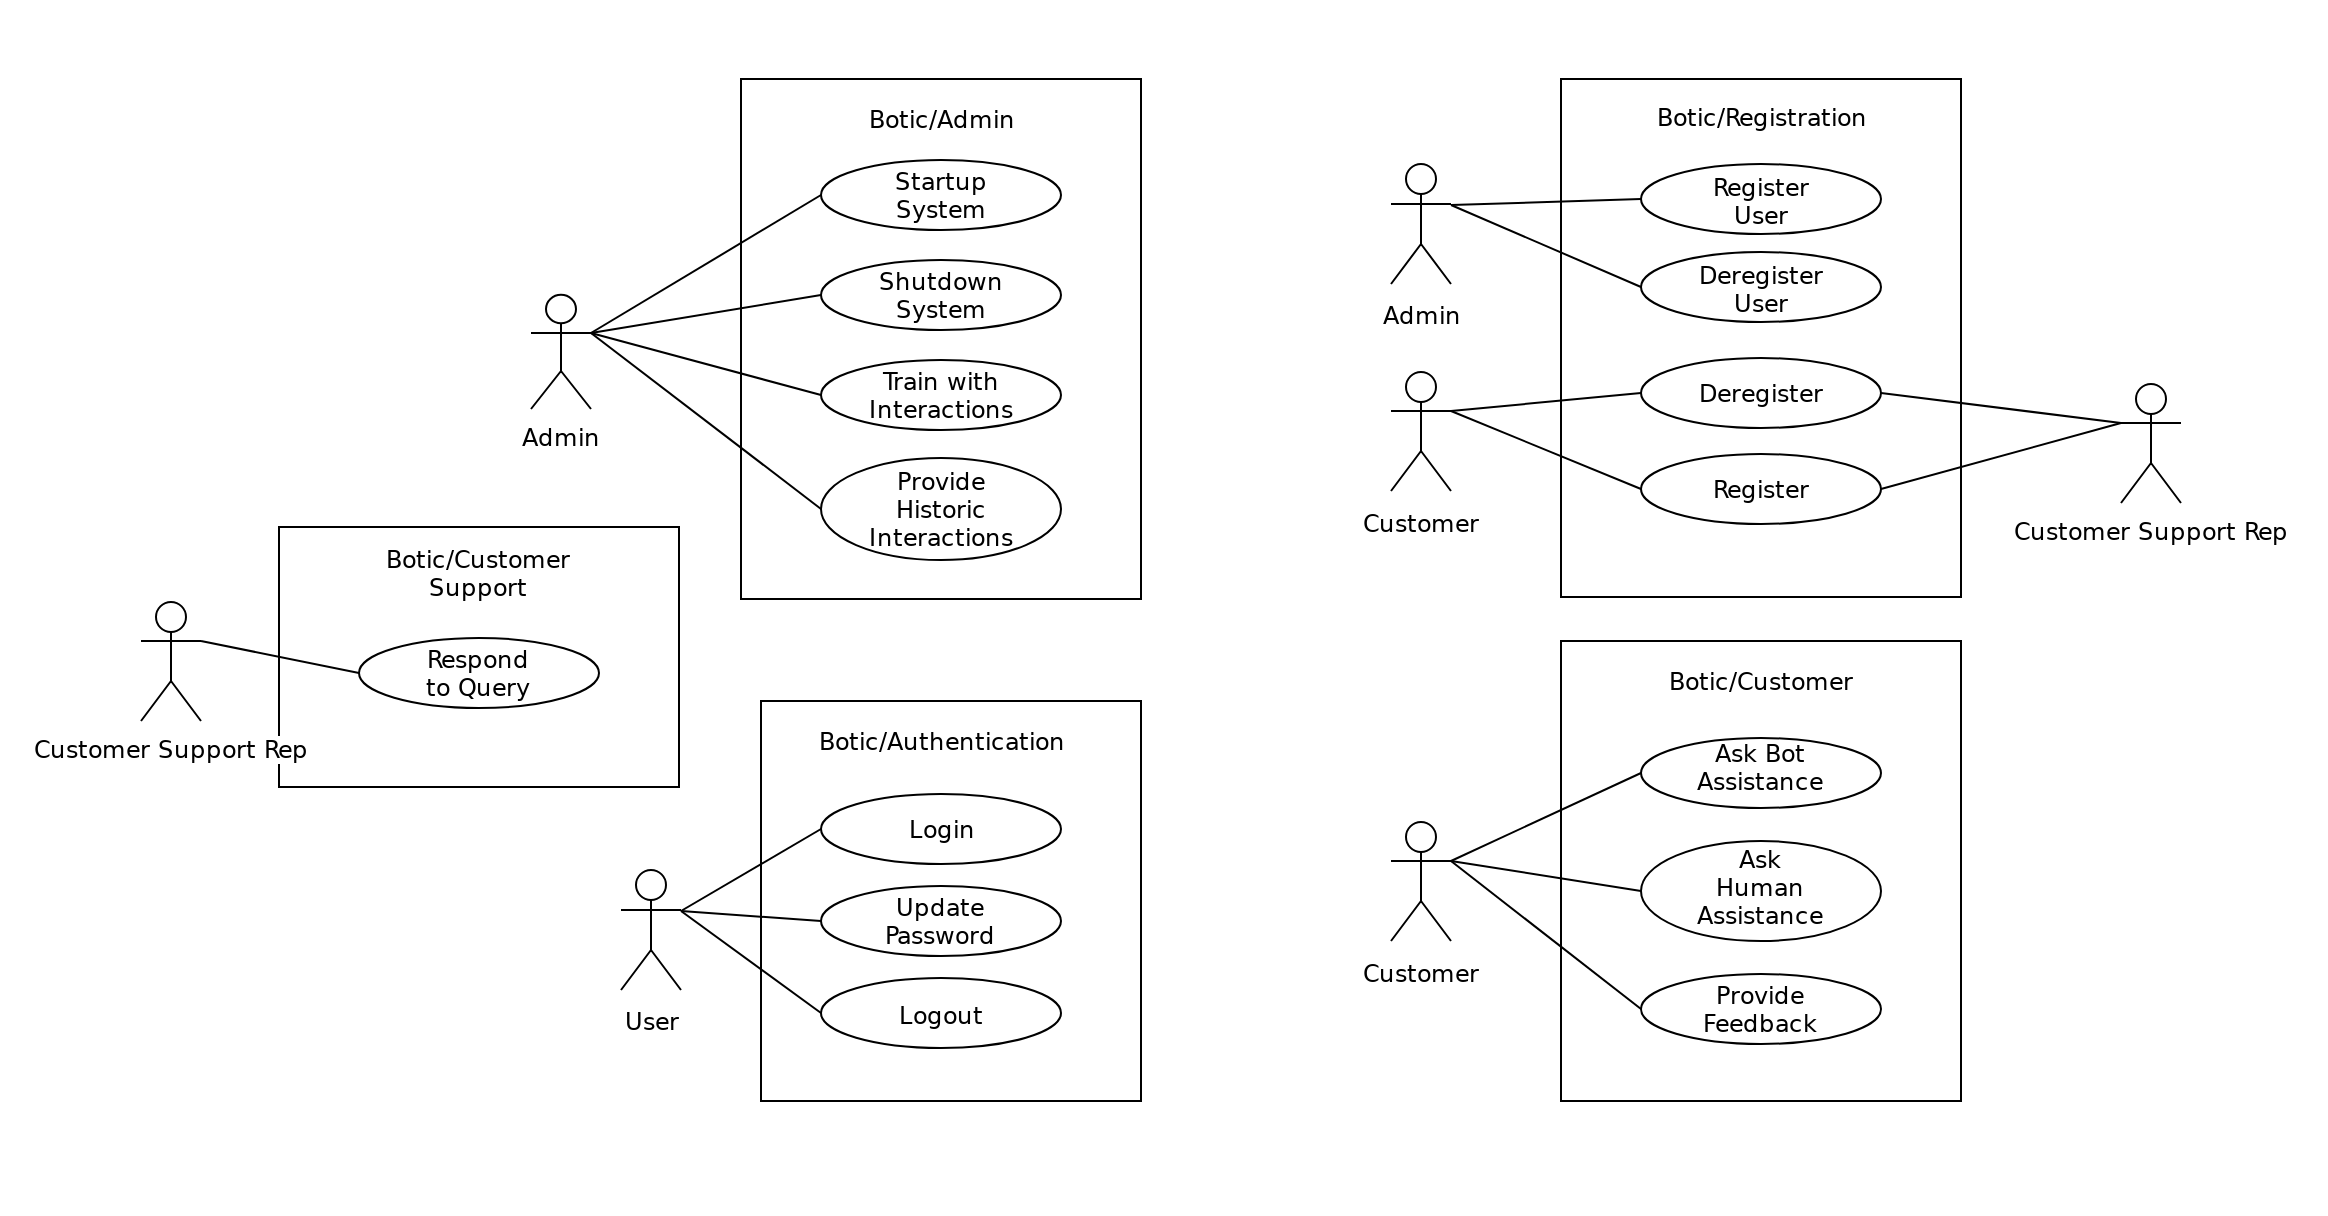
\includegraphics[width=1.2\textwidth]{../../images/Botic_Use_Case_Context_Diagrams.png}
	\caption{Use Case Contexts}
\end{figure}

\subsubsection{Reviewing Use Case Specifications}

All items in the use case review checklist on page 190 in book\cite{Book:1} have been checked, all pass.

\subsubsection{Allocating the Use Cases to Iterations}

The agile method of effort estimation has been used here. Highest point is 5 and the lowest is 1. Let us assume for now, that the team is capable of handling the amount of work in each use case.
%It is enough to have reasonable effort estimation points at the moment; this section should be reviewed and fixed after the demo.
%The priorities of the use cases have to be updated as well to produce some reasonable values.

\begin{center}
	\hspace*{-1.8cm}\begin{tabular}{|c|c|p{2.4cm}|p{1.2cm}|p{1.8cm}|p{1.8cm}|p{1.8cm}|p{1.8cm}|p{1.8cm}|p{1cm}|}
	\hline
	Use Case & Priority & Effort (Agile) & Depend On & Iteration-1  1wks 05/29/19 - 06/03/19 & Iteration-2 3wks 06/06/19 - 06/24/19 & Iteration-3 2wks 07/08/19 - 07/19/19 & Iteration-4 3wks 07/22/19 - 08/09/19 & Iteration-5 2wks  08/12/19 - 08/23/19 & IT-6 2.5wks 08/26/ - 09/11/\\
	\hline
	UC1 & 5 & 4 & None & & & & 4 & & \\
	\hline
	UC2 & 5 & 4 & UC1 & & & & 4 & & \\
	\hline
	UC3 & 5 & 5 & UC9 & 1 & 1 & 1 & 1 & 1 & \\
	\hline
	UC4 & 5 & 3 & UC6 & & & & 1 & 2 & \\
	\hline
	UC5 & 5 & 3 & UC4 & & & & 1 & 2 & \\
	\hline
	UC6 & 4 & 2 & UC3 & & & & 2 & & \\
	\hline
	UC7 & 4 & 5 & UC8 & & & 2 & 2 & 1 & \\
	\hline
	UC8 & 4 & 4 & None & & & & 2 & 2 & \\
	\hline
	UC9 & 5 & 2 & UC13 & 1 & 1 & & & & \\
	\hline
	UC10 & 5 & 1 & UC9 & 1 & & & & & \\
	\hline
	UC11 & 4 & 2 & UC14 & 1 & 1 & & & & \\
	\hline
	UC12 & 4 & 1 & UC11 & 1 & & & & & \\
	\hline
	UC13 & 4 & 2 & None & 2 & & & & & \\
	\hline
	UC14 & 4 & 2 & None & 2 & & & & & \\
	\hline
	UC15 & 4 & 2 & UC13 & 2 & & &  &  & \\
	\hline
	UC16 & 4 & 2 & None & 2 & & &  & & \\
	\hline
	UC17 & 3 & 2 & UC16 & 2 & & & & & \\
	\hline
	UC18 & 4 & 2 & UC13 & & & 2 & & & \\
	\hline
	UC19 & 4 & 2 & UC11 & & & 2 & & & \\
	\hline
	%start here
	UC20 & 3 & 2 & UC21 & & & 2 & & & \\
	\hline
	UC21 & 4 & 2 & None & 2 & &  & & & \\
	\hline
	UC22 & 4 & 2 & None & 2 & & & & & \\
	\hline
	Total Effort &  & 56 & & 19 & 3 & 9 & 17 & 8 & \\
	\hline
	\end{tabular}
\end{center}

\subsection{Allocating Use Cases and Subsystems to Iterations}

\subsection{Producing an Architecture Design}
 %- Links to relevent documentation
%- Special consideration should be made during modeling and analysis to show resources that need protection and entities that access those resources
%- Apply security patterns and security design principles to ensure that security requirements are satisfied.
%- security test plan to guide the security test process

"The design process needs to be performed recursively down the hierarchy until the leaf node components are relatively easy to design and implement." - \cite{Book:1}

In producing the architecture design of the system we will follow the architectural design process outlined in \cite{Book:1}'s chapter 6.3 as well as additional considerations brought forth by our Software Engineering classes and recommended material in SWEBOK (Software Engineering Body of Knowledge) version and \cite{Book:2}. Agile principles will be followed, thus we intend to cover just enough of what is needed. Here we will cover: Design objectives; System Type; Architectural Style; Subsystem functions, interfaces, and interaction behaviour; and lastly, we will review the architectural design.

\subsubsection{Design Objectives}

The system quality attributes outline the essense of the business objectives and priorities of the system. Stated in order, they are: Availability, Security, Reliability, Performance, Scalability and Maintainability. Our design objectives are to achieve these quality attributes, in priority, in serving the responsibilities of the system. 

In order to achieve these quality attributes architectural tactics, which are "techniques an architect can use to achieve the required quality attributes"\cite{Book:2}, will be used. These tactics will then be used to form the architectural design in a manner resembling "first principles." 

\paragraph{Availability}
Looking at the quality attributes involving availability and following the design checklist for availability as specified by \cite{Book:2}, we realise that in order to fascilitate the application of tactics that improve availability, we would have to include the following into our system:
\begin{itemize}
	\item[] 1. Logging of faults
	\item[] 2. Notifying appropriate entities of the faults
	\item[] 3. Disable the source of events causing the fault
	\item[] 4. Be temporarily available if need be
	\item[] 5. Fix or mask the fault/failure
	\item[] 6. or Operate in a degraded mode
\end{itemize}

In order for these to be effected, faults need to be detected, the system needs to be able to recover from faults, and it is appropriate to have a measure of preventing faults before they happen.\\*

In order to log faults, the fault detection mechanism or tactic need to be able to store the detected 'faulty' state. The memento design pattern would clearly be useful here. We can even go as far as to have types of faults being associated with the types of mechanisms set out to identify each. For these, we may apply the Abstract Factory Pattern in order to produce specific fault logs, and store them in our fault logging database through the memento pattern. Event's can be stored in this way, so that we may be able to have a trace of operations that led to an error.\\*

Once that is stored in the caretaker, which in and of itself is a state change, we notify the module responsible for notifying the relevant parties of faults in the system. In order to effect these responsibilities, we would have to assign functionality that stores fault logs, and notifies users. These will be done in reference to use cases, because availability is an attribute that affects users - which are the actors in the use cases. The fault detection mechanisms (architectural tactics) depend on the particular operations of the modules, thus each of the modules or subsystems stand to have their own fault detection mechanisms (availability architectural patterns). This logic applies to tactics responsible for recovering from faults, and preventing faults.\\*

The table below provides the subsystems yeilded from functional clusters for high cohesion, and their system types as well as our chosen fault detection tactic, recovery tactic and fault prevention tactic. These are only subsystems that are necessary, and ordered according to priority. The architectural tactics are solution specific, therefore we expect to add many more of them as the development of the project continues; software engineering is a wicked problem afterall:

\begin{center}
	\hspace*{-1.2cm}\begin{tabular}{|c|c|c|c|c|}
		\hline
		Subsystem & Subsystem Type & Fault Detection & Recovery from Faults & Fault Prevention \\
		\hline
		Chatbot Subsystem & Transformational Subsystem & ping/echo, Retry & Exception Handling & Removal from Service\\
		\hline
	\end{tabular}	
\end{center}
Please note that the Chatbot Subsystem consists of the Message Scraper, Classifier and the Response Generator subsystems; thus all the mentioned tactics actually apply to each of this subsystem's components.

Two modules will be produced here: one for log management, and another for notification. These require that data be persisted.

\paragraph{Security}
Looking at the quality requirements involving security in following the design checklist specified by \cite{Book:1}, we find that it is useful to use physical security as a model for software security as indicated by \cite{Book:2}. This results in the four categories of focus for this quality attribute: detect, resist, react, and recover. \\*

In order to support the design and the analysis of security in our system we will pay attention to the following, and ensure that these responsibilities are assigned and met:
\begin{itemize}
	\item[] 1. Identify the actor
	\item[] 2. Authenticate the actor
	\item[] 3. Authorize actors
	\item[] 4. Grant or deny access to data or services
	\item[] 5. Record attempts to access or modify data or services
	\item[] 6. Encrypt data
	\item[] 7. Recognize reduced availability for resources or services and inform appropriate personnel and restrict access
	\item[] 8. Recover from an attack
	\item[] 9. Verify checksums and hash values
\end{itemize}
 With regards to our data we shall ensure that the following is observed:
\begin{itemize}
	\item[] 1. Seperation of data of different sensitivities
	\item[] 2. Ensure different access to data of different sensitivities
	\item[] 3. Ensure that access to sensitive data is logged and that the log files is suitably protected
	\item[] 4. Ensure that data is suitably encrypted and that keys are separated from the encrypted data
	\item[] 5. Ensure that data can be restored if it is inappropriately modified
\end{itemize}

This attribute modifies or enhances modules introduced in the availability requirement analysis above, this includes the assignment of new responsibilities in particular, certain logs have to be stored securely-- those logging access to sensitive information. It also makes use of the notification module to let the appropriate personnel know that their system is being attacked, when these attacks are detected.\\*

The table below includes the architectural tactics we will employ with respect to each of the four categories (detection, resistance, reaction, and recovery) we defined earlier, the subsystems and their subsystem types. These are in order of priority:
\begin{center}
	\hspace*{-1.5cm}\begin{tabular}{|p{3cm}|p{3cm}|p{3cm}|p{3cm}|p{3cm}|p{3cm}|}
		\hline
		Subsystem & Subsystem Type & Detection & Resistance & Reaction & Recovery \\
		\hline
		User Interface Subsystem & Interactive Subsystem & Detect service denial, Detect message delay & Identify actors, Authenticate actors, Authorize actors, Encrypt data, Separate entities & Revoke access, Lock computer, Inform Actors & Maintain Audit Trail \\
		\hline
		Chabtot Subsystem & Transformational Subsystem & Verify Message Integrity, Detect service denial & Identify actors, Authorize actors, Encrypt data & Revoke access, Inform Actors & Maintain Audit Trail \\
		\hline
		Chatbot Trainer Subsystem & Transformational Subsystem & & Authorize actors, Encrypt data & Inform Actors & Maintain Audit Trail, Data Model checklist above* \\
		\hline
		Database Subsystem & Database subsystem & & Authorize actors, Encrypt data, Separate entities & Inform Actors & Maintain Audit Trail, Data Model checklist above* \\
		\hline
	\end{tabular}
\end{center}
Note: we mention the UI subsystem, but what we really mean are the operations performable by the roles of Administrator and Customer Representative. The UI is how they interact with the system.

These are not meant to be exhaustive; they are meant to be revised according to future needs and adapted with feedback.

\paragraph{Reliability}
All of these concerns are encapsulated in the availability analysis above as well as the security analysis above. The requirements have nonetheless been associated with the revelant use cases.

\paragraph{Performance}
Here we will look at design decisions that affect the performance of the system. Here we will consider two contributors to the response time: processing time and blocked time\cite{Book:2}. In these our architectural tactics will be concerned with the control of resource demand as well as the management of resources. \\*

A design checklist proposed by \cite{Book:2} suggests useful design considerations for the sake of ensuring performance; other than just following this checklist as in, on pages 142 to 144, we will note especially that under resource management, it is advised that we manage and monitor important resources under normal and overloaded operation; resources such as process and thread models-- a detail that involves the availability quality attribute. \\*

The table below includes the architectural tactics that we will employ with respect to the control of resource demand and the management of resources in our system. This will only be for the performance critical components, and ordered by importance. The list contains the following columns: subsystem, subsystem type, control resource demand, and manage resources. This is not an exhaustive list, but alas software engineering is a wicked problem:
\begin{center}
	\hspace*{-1.5cm}\begin{tabular}{|c|c|p{5cm}|p{6cm}|}
		\hline
		Subsystem & Subsystem Type & Control Resource Demand & Manage Resources \\
		\hline
		Chatbot Subsystem & Transformational Subsystem & Prioritize Events, Increase resource efficiency, Reduce overhead & Increase resources*, Introduce concurrency, Load balancer, Schedule resources \\
		\hline
		Message Scraper & Transformation Subsystem & Prioritize Events, Increase resource efficiency & Increase resource*, Introduce concurrency, Load balancer, schedule resources \\
		\hline
	\end{tabular}
\end{center}
Note: With regards to "Increase resources" we mean to say that a recommended deployment environment ought to be a cloud platform such as PaaS (Platform as a Service) which would dynamically increase or reduce resources based on demand and bill the customer accordingly.

\paragraph{Scalability}
Looking into design decisions affecting scalability, we have to consider the impact of adding or of removing resources, and these measures will reflect on associated availability as well as the load that will be assigned to existing and new resources\cite{Book:2}. Here, two kinds of scalability will be dealt with: horizontal scalability (adding more resources to individual units), vertical scalability (adding more resources to individual nodes).\\*

%This quality attribute places emphasisr on the resources of the system; these were placed under special attention during the analysis of the performance attribute especially when it came to introducing concurrency. As an unqualified note, all of the scheduling data structures will have have their data split by some acceptable policy and the load balancers will have to be reconfigured to account for new nodes.

\paragraph{Maintainability}

Maintainability may encapsulate some aspects of modifiability as well as testability and availability. All three of these will be observed as well as that which is required for maintanence management from \cite{Book:1}. \\*

In as far as modifiability is concerned, our architectural tactics in this regard, concern all of our system and its subsystems; they are reducing the size of modules through spliting modules, increasing cohesion by increasing semantic coherence, reducing coupling by encapsulation, using an intermediary, restrict dependencies, refactoring and abstract common services. \\*

Looking at architectural tactics for testability we are mostly going to rely on language specific testing tools, especially those that can allow us to follow state, pause and playback tests. It is also useful to follow documentation. The high priority subsystems, in terms of availability and functional responsibilities are high priorities for testing. \\*

Availability has already been covered above. As far as preparing the system for maintainability is concern, during development we will pay close attention to the application of software design principles as well as the application of software design patterns.

"An aspect of testing in that arena is logging of operational data produced by the system, so that when failures occur, the logged data can be analyzed in the lab to try to reproduce the faults."\cite{Book:2}

\subsubsection{Determine System Types}
%This ought to be done in layers i.e. first layer of granularity

From a top view of the entire system, we have observed that the system is more of an interactive system type. Our system is focused on the customer's interaction with the Chatbot, the customer support's interaction, and the administrator's interaction. This means that the interaction begins and ends with each user. The results in the ordering of all subsystems into a number of layers. This has the consequence of creating a clear and well-documented separation of concerns\cite{Book:2}. 

The layers that result are the following:
\begin{enumerate}
	\item The User Interface Layer
	\item The Chatbot Layer
	\item The Training Layer
	\item The Persistance Layer
\end{enumerate}
*This comes from the application of a 4-Tier Architecture.

These four layers we treat as the total system's four main subsystems. Each of these layers, or subsystems, produce exhibit system types of their own. Going into each, we will apply the architectural design process until the we find that the individual leaf node elements are relatively easy to design and implement\cite{Book:1}. \\*

Now we have a look at the "User Interface Layer." This layer deals heavily with actor requests and responses; all actors primarily interact with this subsystem in order satisfy business processes. This is clearly an interactive subsystem.\par

Looking at the Chatbot layer, we observe that the layers in a transformational subsystem. The Support layer, or rather the Training layer we observe a transformational subsystem. The Perisistance Layer, however, is very clearly an object-persistence subsystem.

\subsubsection{Applying Architectural Styles}
%for each system and subsystem have a look how each design decision made with respect each quality attribute affects each architectural style chosen

\paragraph{Entire System}
The whole system adheres to the 4-Tier architectural style. It's layers or subsystems include: The User Interface Layer, the Chatbot Layer, the Support/Training Layer, and lastly the Persistence Layer. This architectural style ensure that all the subsystems and modules can be seperate and thus developed seperately with minimal interaction between them (changes), ensuring adherance to the software design principles of high cohesion and low coupling\cite{Book:2}. This makes our entire system more portable and modifiable (and thus maintainable). Here is the solution:

\begin{figure}[H]
	\centering
	\hspace*{-2.1cm}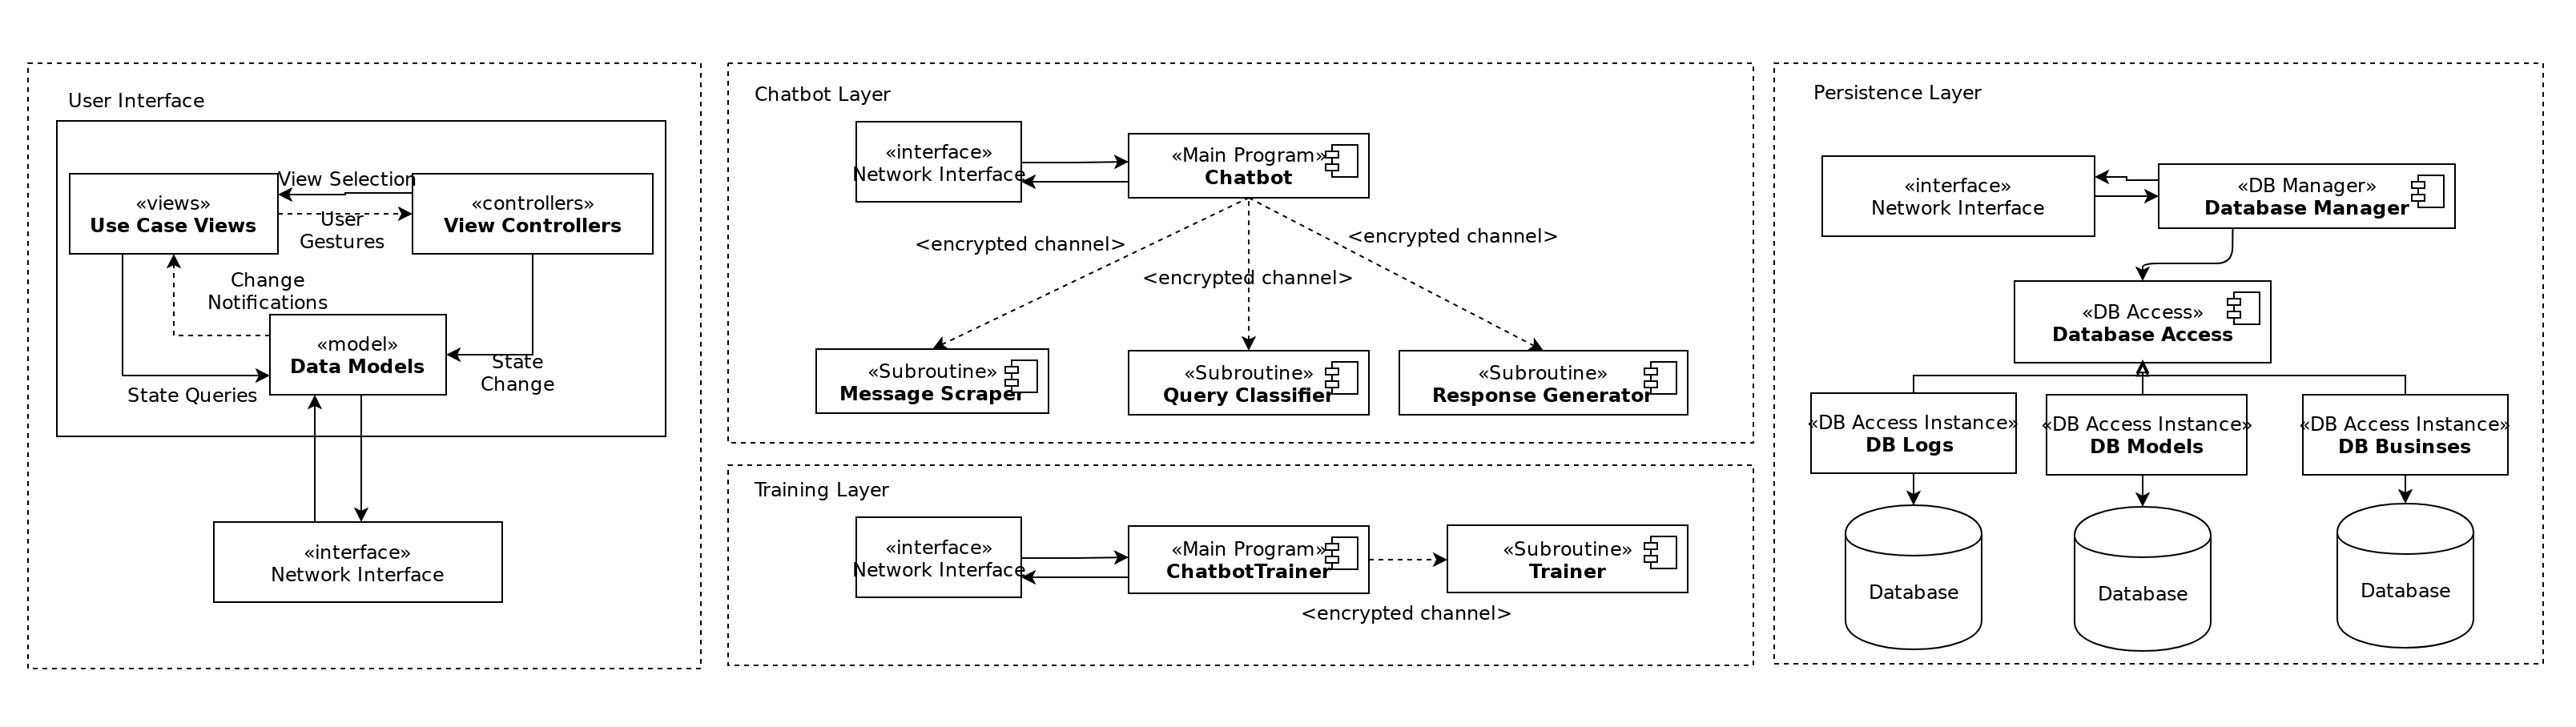
\includegraphics[width=1.25\textwidth]{../../images/Botic_Layered_Architecture.png}
	\caption{Architectural Stye of the System}
\end{figure}

The allowed-to-use relation here is denoted by the geometric adjacency of the layers from left to right-- layers on the left use layers on the right and the layers on the right are used by the layers on the left ONLY. The connections between each layer are made to be through encrypted channels. An appropriate technology will be used to implement this during the implementation phase e.g. SSL.

\paragraph{The User Interface Subsystem}
The User Interface Layer that is also an interactive subsystem uses an MVC architectural style. Using this architectural style, we ensure that user interface interface functionality, something that tends to change frequently especially in response to knew design trends *Quote IMY theory notes, be kept seperate from the application functionality and yet be ever responsive to user input, the most important thing in an interactive system\cite{Book:2}. This is the solution:

\begin{figure}[H]
	\centering
	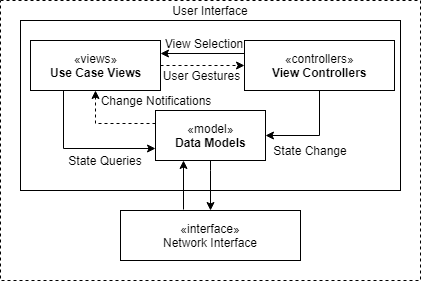
\includegraphics[width=0.5\textwidth]{../../images/User_Interface_MVC.png}
	\caption{Architectural Style of the User Interface}
\end{figure}

\paragraph{The Chatbot Layer}
The Chatbot Layer is a transformational subsystem, and will use a Main Program and Subroutines architectural style.

\begin{figure}[H]
	\centering
	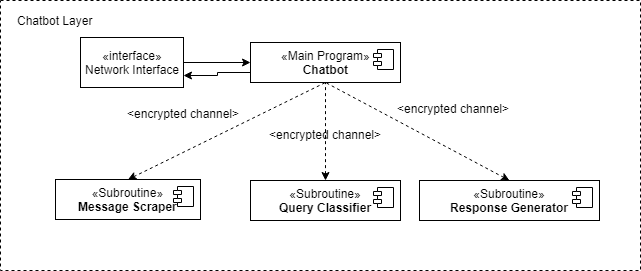
\includegraphics[width=0.8\textwidth]{../../images/Chatbot_Layer_Architecture.png}
	\caption{Architectural Style of the Chatbot Layer}
\end{figure}

\paragraph{The Training Layer}
This layer is a transformational subsystem and will also use a Main Program and Subroutines architectural style.

\begin{figure}[H]
	\centering
	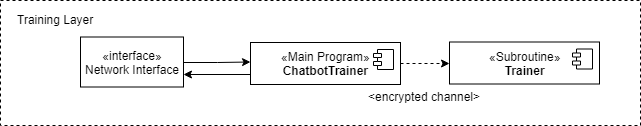
\includegraphics[width=0.8\textwidth]{../../images/Training_Layer_Architecture.png}
	\caption{Architectural Style of the Training Layer}
\end{figure}

The ChatbotTrainer is a single container that has 4 instances: these are to service requests from the user interface (requests which are sent by the Administrator user), one to train the Message Scraper, one to train the Classifier, and one to train the Response Generator. It uses the Strategy Desgin Pattern to switch different training strategies/methods to suit each subsystem it services. This results in multiple instances of the same subsystem, but each using a different training method and data on a different chatbot subsystem.

\paragraph{The Persisitance Layer}
This layer is a clear candidate for the Persistence Framework architectural style, and it's architectural style is just that. Here is our solution:

\begin{figure}[H]
	\centering
	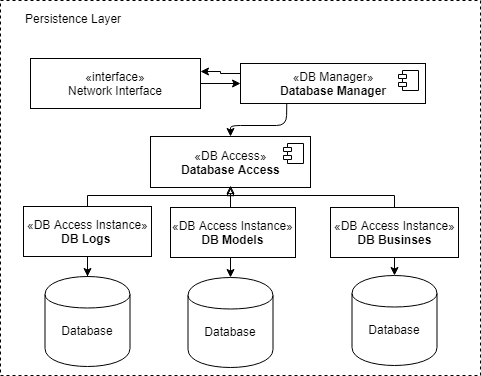
\includegraphics[width=0.6\textwidth]{../../images/Persistence_Layer_Architecture.png}
	\caption{Architectural Style of the Persistence Layer}
\end{figure}

In accordance to the architectural tactics we have chosen to observe to achieve availability and security quality attributes and requirements, in particular the security tactic to seperate access and data of different sensitivities, we have made the decision to have three databases. The first is for logs and audit trails, the second for the data models what would be used for the chatbot subsystems, and the third for recording queries and responses-- data that is concerned with the functional business processes.

\section{Iterative Phase}

%Important to go through the quality attributes and develop their use cases i.e. security: misuse cases
%Important to indicate how we used knowledge gained from all of our modules in university (capstone project)

%Interative Phase:
%- All artifacts are listed and the changes can be checked out by cross referencing appropriate artifacts.
%- Each phase should logically include changes to all the implementation documentation.
%- Special consideration should be made during modeling and analysis to show resources that need protection and entities that access those resources
%- Practice secure coding to ensure that security principles and security patterns are applied to produce secure code during the implementation phase-- use quality assurance reviewing to make sure of this.
%- Also test for security-- test for each quality requirement really; apply static and dynamic security testing. Functional testing, security test
%- Domain modeling should identify and capture security related domain concepts and relationships like the roles and resources accessed by the roles as well as related access priviledges
%- Design for security and other non functional requirements important during actor-system interaction modeling

\subsection{Phase 1:}
%- Demo 1 happened here.
%- Phase 2 artifacts to be listed here.

\subsubsection{Accomodating Requirements Change}
 
\subsubsection{Domain Modeling}

\begin{figure}[H]
	\centering
	\hspace*{-1.7cm}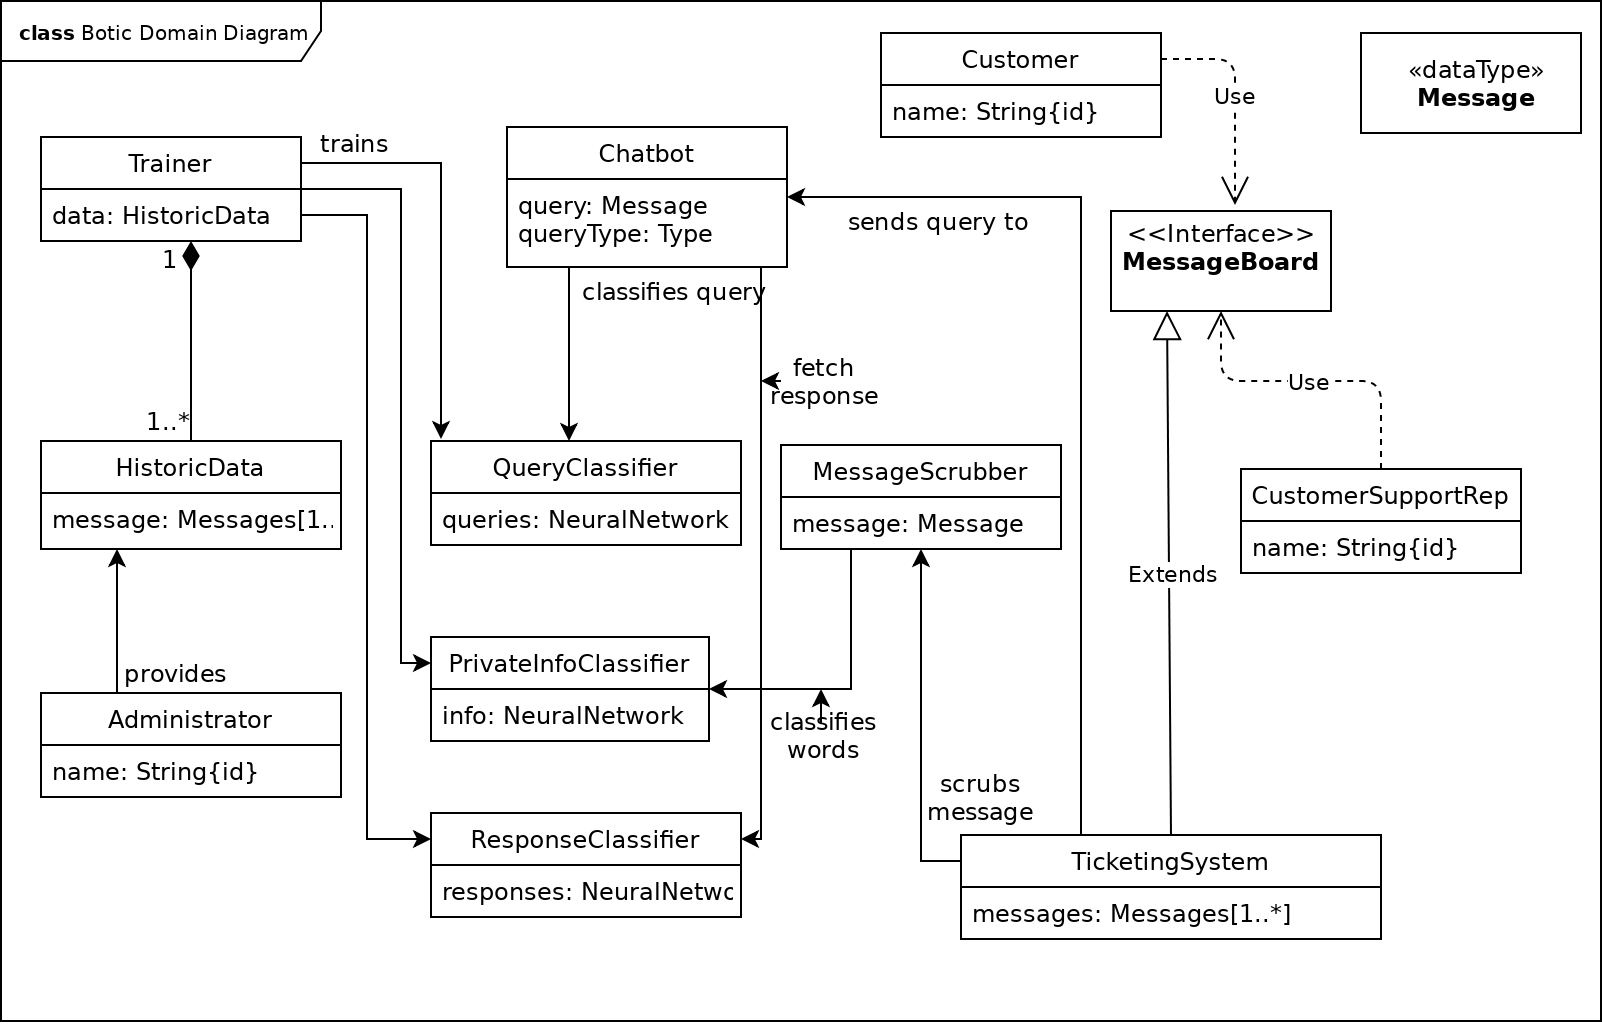
\includegraphics[width=1.2\textwidth]{../../images/Botic_Domain_Diagram.png}
	\caption{UML Domain Model of the Botic System}
\end{figure}
 
\subsubsection{Actor-System Interaction Modeling and User Interface Design}

\paragraph{Actor-System Interaction Modeling}

\begin{table}[h!]
	\centering
	\begin{tabular}{|p{8cm}|p{8cm}|}
		\hline
		Actor: Administrator & System: Authentication \\
		\hline
		 & 0. The System displays the home page.\\
		\hline
		1. TUCBW the administrator clicking the "Sign In" button on the home page. & 2. The accordingly displays the login page.\\
		\hline
		3. The admin (a) enters their Email address and password and clicks "Log In" (b) clicks on an appropriate Single Sign On option. & 4. The system displays (a) an "incorrect login" error message (b) a "correct login" details message. \\
		\hline
		5. TUCEW the administrator being redirected to the Botic Admin page. & \\
		\hline
	\end{tabular}
	\caption{UC21. Login}
\end{table}

\begin{table}[h!]
	\centering
	\begin{tabular}{|p{8cm}|p{8cm}|}
		\hline
		Actor: Administrator & System: Authentication \\
		\hline
		 & 0. The System displays Botic Admin page.\\
		\hline
		1. TUCBW the administrator clicking the "Sign Out" button on the Botic Admin page. & 2. The system clears the admin's current session and logs them out. \\
		\hline
		3. TUCEW the administrator being redirected to the home page. & \\
		\hline
	\end{tabular}
	\caption{UC22. Logout}
\end{table}
 
\begin{table}[h!]
	\centering
	\begin{tabular}{|p{8cm}|p{8cm}|}
		\hline
		\multicolumn{2}{|c|}{Precondition: The Administrator must have logged in.} \\
		\hline
		Actor: Administrator & System: Authentication \\
		\hline
		 & 0. The System displays the Botic Admin page.\\
		\hline
		1. TUCBW an Admin clicks on the "Register User" button on the Botic Admin page. & 2. The system prompts the admin for all necessary details for the user being registered. \\
		\hline
		3. The Admin clicks the "Confirm Registration" button. & 4. The system registers the user and sends them an Email to update their password, along with a randomly generated password. \\
		\hline
		5. TUCEW the Admin receives the message "User Has Been Registered." & \\
		\hline
		\multicolumn{2}{|c|}{Postcondition: NONE} \\
		\hline
	\end{tabular}
	\caption{UC16: Register User}
\end{table}

\begin{table}[H]
	\centering
	\begin{tabular}{|p{8cm}|p{8cm}|}
		\hline
		\multicolumn{2}{|c|}{Precondition: The Administrator must have logged in.} \\
		\hline
		Actor: Administrator & System: Authentication \\
		\hline
		& 0. The System displays the Botic Admin page. \\
		\hline
		1. TUCBW an Admin clicking on the "Deregister User" button on the Botic Admin page. & 2. The system displays all users in three columns according to their user types i.e. customer, customer support representative, admin.\\
		\hline
		3. The administrator clicks on the delete icon next to the appropriate user & 4. The system (a) deletes the user from the system, (b) sends a deletion confirmation to the admin being deleted. \\
		\hline
		5. (a) TUCEW the Admin recieves the message "User Has Been Deregistered.", (b) TUCEW the Admin recieving the message "Deletion Request Sent." & \\
		\hline
		\multicolumn{2}{|c|}{Postcondition: NONE} \\
		\hline
	\end{tabular}
	\caption{UC17: Deregister User}
\end{table}
 
\begin{table}[H]
	\centering
	\begin{tabular}{|p{8cm}|p{8cm}|}
		\hline
		Actor: Customer & System: Authentication \\
		\hline
		 & 0. The System displays the home page.\\
		\hline
		1. TUCBW the customer clicking the "Sign In" button on the home page. & 2. The accordingly displays the login page.\\
		\hline
		3. The customer (a) enters their Email address and password and clicks "Log In" (b) clicks on an appropriate Single Sign On option. & 4. The system displays (a) an "incorrect login" error message (b) a "correct login" details message. \\
		\hline
		5. TUCEW a customer gets redirected to the customer chat page (and it is opened). & \\
		\hline
	\end{tabular}
	\caption{UC9: Login}
\end{table}

\begin{table}[h!]
	\centering
	\begin{tabular}{|p{8cm}|p{8cm}|}
		\hline
		Actor: Customer & System: Authentication \\
		\hline
		 & 0. The System displays the customer chat page.\\
		\hline
		1. TUCBW the administrator clicking the "Sign Out" button on the Botic Admin page. & 2. The system clears the customer's current session and logs them out. \\
		\hline
		3. TUCEW the customer being redirected to the home page. & \\
		\hline
	\end{tabular}
	\caption{UC10: Logout}
\end{table}

\begin{table}[h!]
	\centering
	\begin{tabular}{|p{8cm}|p{8cm}|}
		\hline
		Actor: Customer Support Representative & System: Authentication \\
		\hline
		 & 0. The System displays the home page.\\
		\hline
		1. TUCBW the customer support rep. clicking the "Sign In" button on the home page. & 2. The accordingly displays the login page.\\
		\hline
		3. The customer support rep. (a) enters their Email address and password and clicks "Log In" (b) clicks on an appropriate Single Sign On option. & 4. The system displays (a) an "incorrect login" error message (b) a "correct login" details message. \\
		\hline
		5. TUCEW a customer gets redirected to the customer support chat page (and it is opened). & \\
		\hline
	\end{tabular}
	\caption{UC11: Login}
\end{table}

\begin{table}[h!]
	\centering
	\begin{tabular}{|p{8cm}|p{8cm}|}
		\hline
		Actor: Customer Support Representative & System: Authentication \\
		\hline
		 & 0. The system displays the customer support chat page. \\
		\hline
		1. TUCBW a customer support representative clicks the "Sigh Out" button on the customer support chat page. & 2. The system clears the customer support rep's current session and logs them out. \\
		\hline
		3. TUCEW a customer support representative gets redirected to the home page. & \\
		\hline
	\end{tabular}
	\caption{UC12: Logout}
\end{table}

\begin{table}[H]
	\centering
	\begin{tabular}{|p{8cm}|p{8cm}|}
		\hline
		Actor: Customer & System: Authentication \\
		\hline
		& 0. The system displays the home page. \\
		\hline
		1. TUCBW a customer clicks on the "Register" button on the home page. & 2. The system (a) prompts the user for their name, Email and password (b) allows them to register via Single Sign On.\\
		\hline
		3. The customer (a) clicks the "Confirm Registration" button, or (b) clicks the relevant profile for Single Sign On. & 4. The system registers the customer and sends a default password via Email to Single Sign On users. \\
		\hline
		5. TUCEW a customer gets the message "You have been Registered" and gets redirected to the home page. & \\
		\hline
	\end{tabular}
	\caption{UC13: Register}
\end{table}

\begin{table}[H]
	\centering
	\begin{tabular}{|p{8cm}|p{8cm}|}
		\hline
		Actor: Customer Support Representative & System: Authentication \\
		\hline
		 & 0. The system displays the home page. \\
		\hline
		1. TUCBW a customer support representative clicks on the "Register" button on the home page. & 2. The system (a) prompts the user for their name, Email and password (b) allows them to register via Single Sign On. \\
		\hline
		3. The customer (a) clicks the "Confirm Registration" button, or (b) clicks the relevant profile for Single Sign On. & 4. The system sends an Email to an Administrator to approve the request along with a link to approve it. It displays a message saying "Registration Pending."\\
		\hline
		5. TUCEW a customer support representative recieves a notification with the message "You have been Approved." & \\
		\hline
	\end{tabular}
	\caption{UC14: Register}
\end{table}


\begin{table}[H]
	\centering
	\begin{tabular}{|p{8cm}|p{8cm}|}
		\hline
		Actor: Customer & System: Authentication\\
		\hline
		 & 0. The system displays the customer chat page. \\
		\hline
		1. TUCBW a customer clicks on the "Deregister" button on customer chat page. & 2. The system prompts the user if they are sure they intend to deregister. \\
		\hline
		3. The customer cofirms deregistration by clicking "Confirm" & 4. The system deletes all relevant data partaining to the customer according to deletion policies.\\
		\hline
		5. TUCEW a customer recieves "Customer profile has been successfully deregistered" message and is redirected to the home page. & \\
		\hline
	\end{tabular}
	\caption{UC15: Deregister}
\end{table}

\begin{table}[H]
	\centering
	\begin{tabular}{|p{8cm}|p{8cm}|}
		\hline
		Actor: Customer & System: Chatbot \\
		\hline
		 & 0. The system displays the customer chat page. \\
		\hline
		1. TUCBW a customer typing a message into the input box in the customer chat page. & 2. The system detects private or personal information as the customer types in their query and warns them if it is detected by highlighting it according to severity. \\
		\hline
		3. The customer clicks the "Send Query" button to send the query to the chatbot & 4. 	The system (a) answers the customer query, or (b) forwards the query to a customer support representative \\
		\hline
		5. TUCCW UC6 to provide feedback and finally TUCEW a customer recieving a "Session has ended" message. & \\
		\hline
	\end{tabular}
	\caption{UC3: Ask Bot Assistance}
\end{table}

\paragraph{User Interface Design}
%this is where you can more readily implement knowledge gained from IMY 320

%guideline 12.1 in chapter 12 of book 1 provides motivation for the use of SPA-- limiting the number of container pages contributes to better user experience.
This stage will make use of the user interface design process outlined by \cite{Book:1}. We begin by identifying major system displays; these and user input and user actions as well as the information displayed are provided in the following tables, each corresponding to a particular expanded use case (produced in the previous step):

\begin{table}[H]
	\centering
	\hspace*{-0.17cm}\begin{tabular}{|p{2cm}|p{3cm}|p{3cm}|p{3cm}|p{5cm}|}
		\hline
		Expanded Use Case Step & System Display & Information Displayed & User Input & User Actions \\
		\hline
		0 & Botic Home Page & & & \\
		\hline
		3 & System Login Page & & Requested Information & i. enters Email address and password, or ii. clicks on Single Sign On option \\
		\hline
		4 & System Login Page & "Incorrect Login Details", "Correct Login (Loading)" & Requested Information & i. enters correct Email address and password, or ii. Clicks to grant permission to use Single Sign On \\
		\hline
	\end{tabular}
	\caption{Major System Displays for the Administrator Login use case}
\end{table}
All login use cases feature the same system displays, information displayed, user input and user actions. Thus, by agile principles, the table above is enough to represent all relevant use cases. The Logout use cases will not be analysed in this manner, they are short and involve a simple button click.

Note: Client feedback has suggested that the user interface is for demo purposes only and is "throw-away." It currently does not involve many elements at all and the moment, thus this would be all for this stage.

\subsubsection{Behavior Modeling and Responsibility Assignment}

\paragraph{Behavior Modeling}

Most of the use cases in this iteration involve the user interface subsystem, which is an interactive subsystem. It is because of this, that the focus of this section will be Object Interaction Modeling which is concerned with the modeling of interactive systems \cite{Book:1}. The Ask Bot Assistance use case has some involvement with the user interface as well as the transformational chatbot subsystem; this means that we may include some activity modeling which is suitable for transformational subsystems according to \cite{Book:1}. Since background processes are being analysed, we may show how the architectural tactics and other design decisions are implemented in the behavior of the system objects.\\*

We will only use sequence diagrams to model the behaviour of our systems during use case execution. This is because sequence diagrams are semantically equivalent to the other interaction diagram, communication diagrams\cite{Book:1}. Because we are a novice team, it is recommended that even though we use agile principles, we ought to follow all the steps of OIM, we however will leave out trivial use cases such as those that are the same for different actors\cite{Book:1}.\\*

The first step has already been fulfilled as information has already been collected and actor-system interaction models for the use cases in this iteration have already been produced. We now focus on identifying the nontrivial steps; which are the step that require background processing i.e. objects in the system to interact and work together to produce a desired result. The following are the use cases we have decided to have their behaviour modelled for this iteration, the nontrivial steps are highlighted:

\begin{table}[h!]
	\centering
	\begin{tabular}{|p{8cm}|p{8cm}|}
		\hline
		Actor: Administrator & System: Authentication \\
		\hline
		 & 0. The System displays the home page.\\
		\hline
		1. TUCBW the administrator clicking the "Sign In" button on the home page. & 2. The accordingly displays the login page.\\
		\hline
		3. The admin (a) enters their Email address and password and clicks "Log In" (b) clicks on an appropriate Single Sign On option. &\cellcolor{blue} 4. The system displays (a) an "incorrect login" error message (b) a "correct login" details message. \\
		\hline
		5. \cellcolor{blue} TUCEW the administrator being redirected to the Botic Admin page. & \\
		\hline
	\end{tabular}
	\caption{UC21. Login}
\end{table}

\begin{table}[h!]
	\centering
	\begin{tabular}{|p{8cm}|p{8cm}|}
		\hline
		\multicolumn{2}{|c|}{Precondition: The Administrator must have logged in.} \\
		\hline
		Actor: Administrator & System: Authentication \\
		\hline
		 & 0. The System displays the Botic Admin page.\\
		\hline
		1. TUCBW an Admin clicks on the "Register User" button on the Botic Admin page. & 2. The system prompts the admin for all necessary details for the user being registered. \\
		\hline
		3. The Admin clicks the "Confirm Registration" button. & \cellcolor{blue} 4. The system registers the user and sends them an Email to update their password, along with a randomly generated password. \\
		\hline
		5. TUCEW the Admin receives the message "User Has Been Registered." & \\
		\hline
		\multicolumn{2}{|c|}{Postcondition: NONE} \\
		\hline
	\end{tabular}
	\caption{UC16: Register User}
\end{table}

\begin{table}[H]
	\centering
	\begin{tabular}{|p{8cm}|p{8cm}|}
		\hline
		\multicolumn{2}{|c|}{Precondition: The Administrator must have logged in.} \\
		\hline
		Actor: Administrator & System: Authentication \\
		\hline
		& 0. The System displays the Botic Admin page. \\
		\hline
		1. TUCBW an Admin clicking on the "Deregister User" button on the Botic Admin page. & \cellcolor{blue} 2. The system displays all users in three columns according to their user types i.e. customer, customer support representative, admin.\\
		\hline
		3. The administrator clicks on the delete icon next to the appropriate user & \cellcolor{blue} 4. The system (a) deletes the user from the system, (b) sends a deletion confirmation to the admin being deleted. \\
		\hline
		5. (a) TUCEW the Admin recieves the message "User Has Been Deregistered.", (b) TUCEW the Admin recieving the message "Deletion Request Sent." & \\
		\hline
		\multicolumn{2}{|c|}{Postcondition: NONE} \\
		\hline
	\end{tabular}
	\caption{UC17: Deregister User}
\end{table}
 
\begin{table}[H]
	\centering
	\begin{tabular}{|p{8cm}|p{8cm}|}
		\hline
		Actor: Customer Support Representative & System: Authentication \\
		\hline
		 & 0. The system displays the home page. \\
		\hline
		1. TUCBW a customer support representative clicks on the "Register" button on the home page. & 2. The system (a) prompts the user for their name, Email and password (b) allows them to register via Single Sign On. \\
		\hline
		3. The customer (a) clicks the "Confirm Registration" button, or (b) clicks the relevant profile for Single Sign On. & \cellcolor{blue} 4. The system sends an Email to an Administrator to approve the request along with a link to approve it. It displays a message saying "Registration Pending."\\
		\hline
		5. TUCEW a customer support representative recieves a notification with the message "You have been Approved." & \\
		\hline
	\end{tabular}
	\caption{UC14: Register}
\end{table}

\begin{table}[H]
	\centering
	\begin{tabular}{|p{8cm}|p{8cm}|}
		\hline
		Actor: Customer & System: Chatbot \\
		\hline
		 & 0. The system displays the customer chat page. \\
		\hline
		1. TUCBW a customer typing a message into the input box in the customer chat page. & \cellcolor{blue} 2. The system detects private or personal information as the customer types in their query and warns them if it is detected by highlighting it according to severity. \\
		\hline
		3. The customer clicks the "Send Query" button to send the query to the chatbot & \cellcolor{blue} 4. 	The system (a) answers the customer query, or (b) forwards the query to a customer support representative \\
		\hline
		5. \cellcolor{blue} TUCCW UC6 to provide feedback and finally TUCEW a customer recieving a "Session has ended" message. & \\
		\hline
	\end{tabular}
	\caption{UC3: Ask Bot Assistance}
\end{table}

Now we continue OIM by writing scenarios for the nontrivial steps. These we will use to produce the UML sequence diagrams. To avoid sequence diagrams that are too lengthly and complex, the methodology we use, the Agile Unified Method, only models the nontrivial steps featured in expanded use cases \cite{Book:1}. As I'm sure you can notice, some nontrivial requests have been highlighted as well, we do this because they involve relevent system activities that may just have only been implied in the nontrivial steps-- it is done for clarity's sake. The following are the use case scenarios for the selected use cases.

\begin{table}[H]
	\centering
	\fcolorbox{black}[HTML]{E9F0E9}{\parbox{\textwidth}{
		\begin{enumerate}[label=3.]
			\item The admin (a) enters their Email address and password and clicks "Log In" (b) clicks on an appropriate Single Sign On option.
		\end{enumerate}
		\begin{enumerate}[label=4.\arabic*.]
			\item The Signin GUI (header widget) signs in with the login controller.
			\item The login controller creates a login log for the user using the IP address of the user and login attempt.
			\item The login controller saves the login log with the Database Manager.
			\item The login controller signs in using the authentication service.
			\item The authentication service authorizes the user using WebAuth.
			\item WebAuth returns an access token to the authentication service.
			\item The authentication service validates the access token using WebAuth.
			\item If the access token is valid
			\begin{enumerate}[label*=\arabic*.]
				\item The authentication service obtains the user profile from WebAuth using the access token.
				\item The authentication service creates a session for the user using access token.
				\item The authentication returns a true login in status to the login controller.
			\end{enumerate}
			\item else, 
			\begin{enumerate}[label*=\arabic*.]
				\item The authenitication returns a failed login status to the login.
			\end{enumerate}
			\item If the login status is true
			\begin{enumerate}[label*=\arabic*.]
				\item The login controller gets the login log from the database manager using the IP address of the user.
				\item If the login log is too old or doesn't exist
				\begin{enumerate}[label*=\arabic*.]
					\item The login controller signs out using the authentication service.
					\item The authentication service clears the session.
					\item If login log doesn't exist
					\begin{enumerate}[label*=\arabic*.]
						\item The login controller returns an "IP address change during login; please login again." message to the Signin GUI.
					\end{enumerate}
					\item else, 
					\begin{enumerate}[label*=\arabic*.]
						\item The login controller returns a "login took too long" message to the Signin GUI. 
					\end{enumerate}
					\item The Signin GUI displays the message.
				\end{enumerate}
				\item else,
				\begin{enumerate}[label*=\arabic*.]
					\item The login controller enters a login success in the login log.
					\item The login controller saves the login log with the Database Manager.
					\item The login controller redirects the user to their appropriate page. 
				\end{enumerate}
			\end{enumerate}
			\item else,
			\begin{enumerate}[label*=\arabic*.]
				\item The login controller redirects the user to the home page. 
			\end{enumerate}
		\end{enumerate}
	}}
	\caption{Use Case Scenario for UC21: Login}
\end{table}
We use Auth0 as a third party authentication server to log users in and return the user token to our system so that we may "sign them in." We interface with Auth0 by using WebAuth.\\*

The scenarios will now be converted into scenario tables. This helps with the conversion from the scenarios to sequence diagrams. The scenario table for use case 21 will not be constructed. The scenario is enough. The methodology specifies that is optional. \\*

The next step is the construction of the sequence diagrams for each use case scenario (and corresponding use case scenario table if it exists). These are the informal sequence diagrams for the chosen use cases:

\begin{figure}[H]
	\centering
	\hspace*{-1.5cm}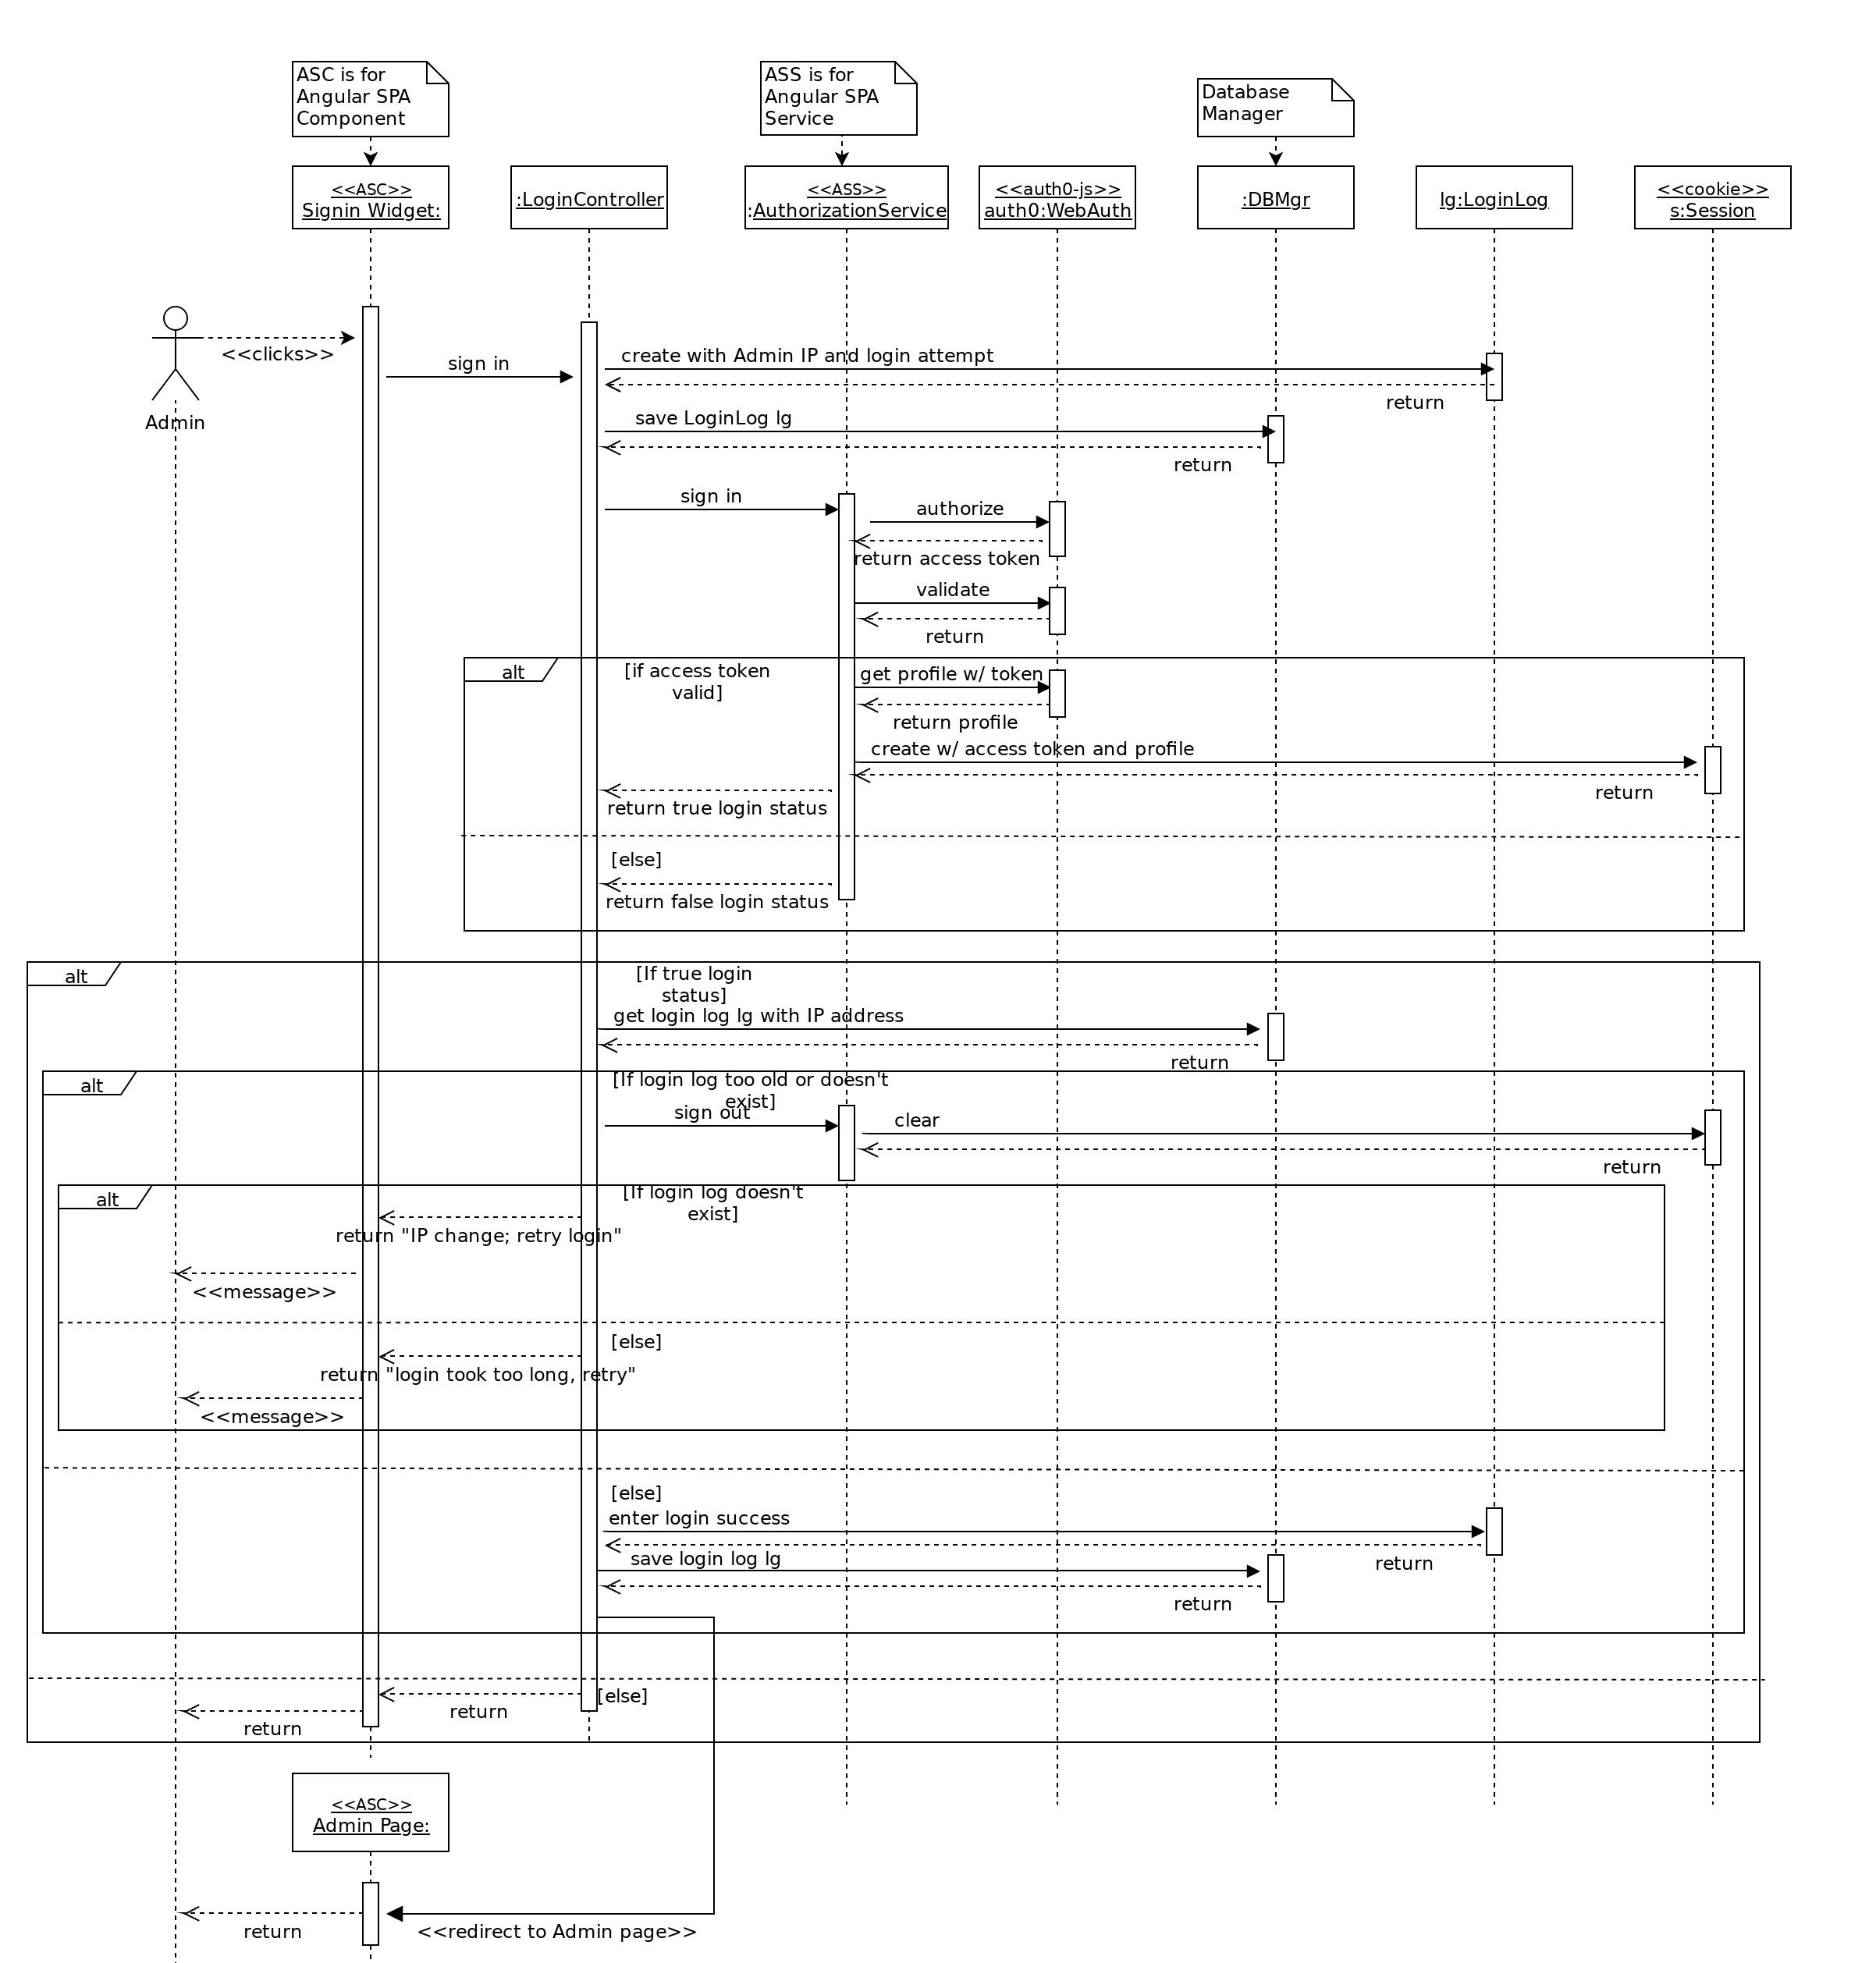
\includegraphics[width=1.2\textwidth]{../../images/Informal_Sequence_Diagram_UC21.png}
	\caption{Informal Sequence Diagram for UC21}
\end{figure}

The next step is to decide on the names as well as the types of the object instances that send as also receive message, we do this as well as determine function names, parameters and return types. This produces designl sequence diagrams. These are the design sequence diagrams of the chosen use cases:

\begin{figure}[H]
	\centering
	\hspace*{-1.5cm}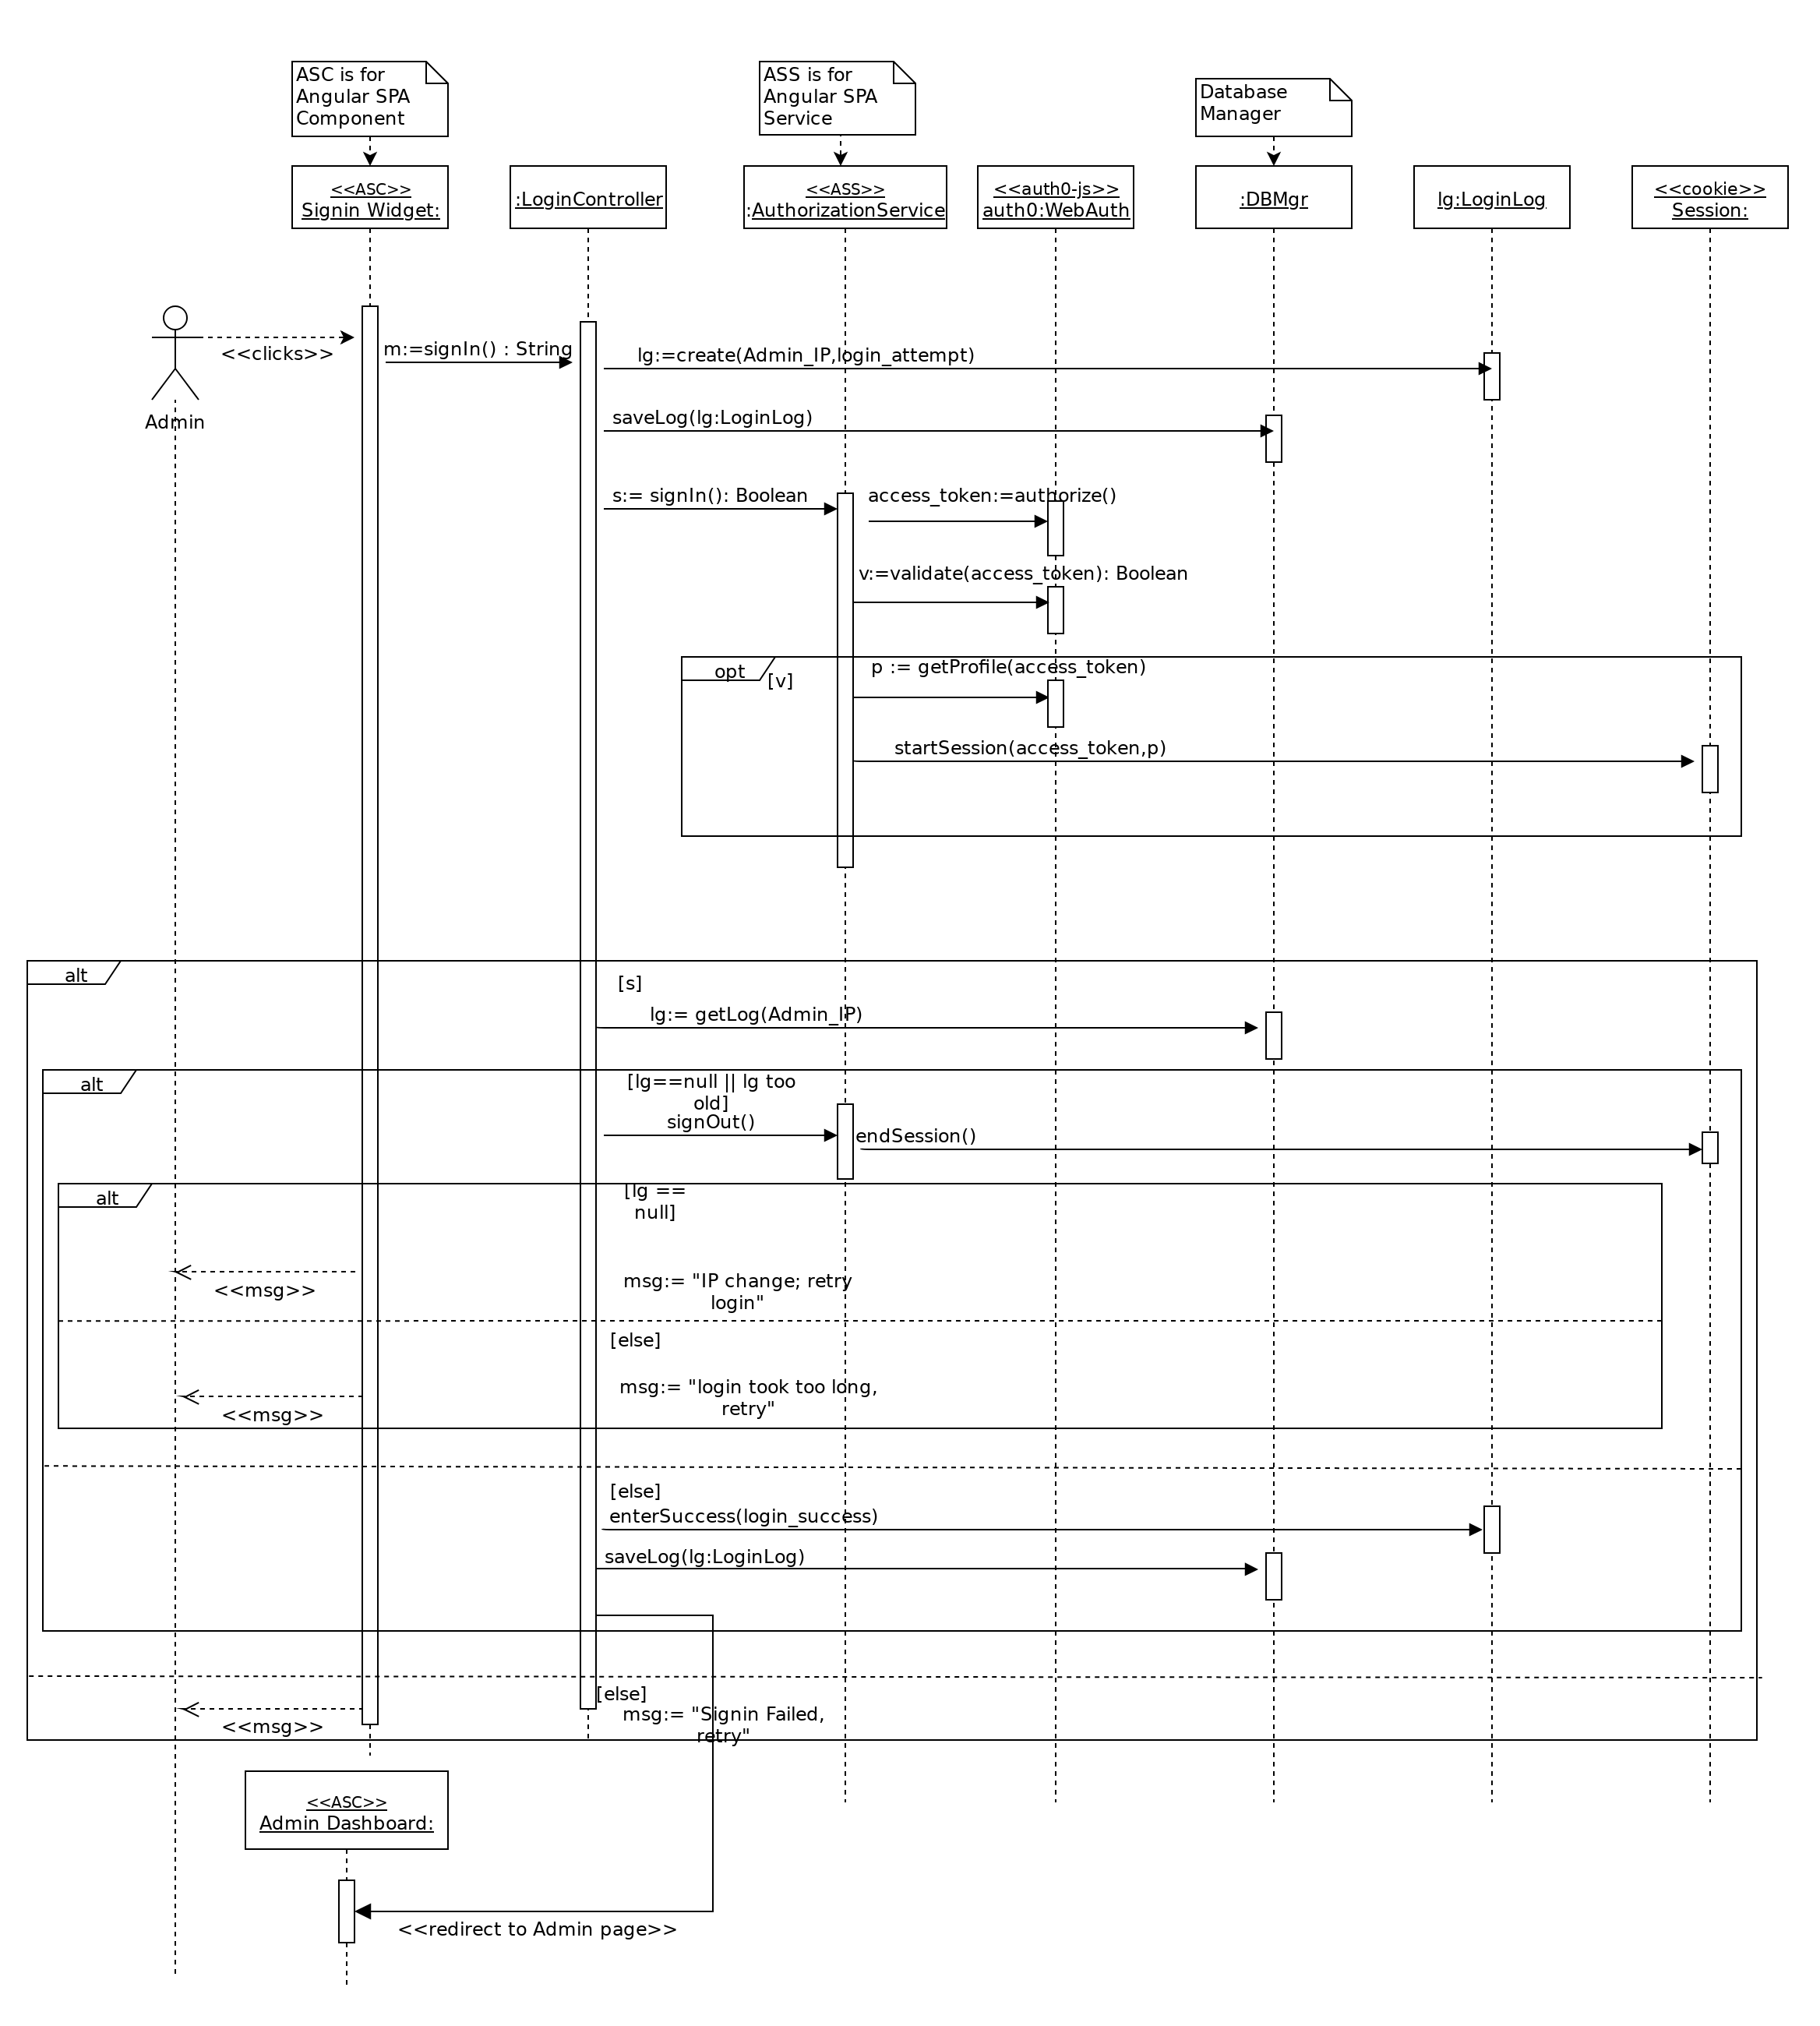
\includegraphics[width=1.2\textwidth]{../../images/Design_Sequence_Diagram_UC21.png}
	\caption{Informal Sequence Diagram for UC21}
\end{figure}

\paragraph{Responsibility Assginment}
 
\subsubsection{Deriving Design Class Diagram}
 
\subsubsection{Test-Driven Development}
 
\subsubsection{Integration}
 
\subsubsection{Deployment}
%Place acceptance testing after this one as well as customer feedback
\subsection{Phase 2:} 
 - Demo 2 happened here
 - Phase 2 artifacts to be listed here.

\subsubsection{Accomodating Requirements Change}
 
\subsubsection{Domain Modeling}
  
\subsubsection{Actor-System Iteraction Modeling and User Interface Design}
  
\subsubsection{Behavior Modeling and Responsibility Assignment}
  
\subsubsection{Deriving Design Class Diagram}
  
\subsubsection{Test-Driven Development}
  
\subsubsection{Integration}
  
\subsubsection{Deployment}

\subsection{Phase 3:}

\subsubsection{Accomodating Requirements Change}
- Another meeting with clients (include proper date).
- Refined the requirements according to proper rules thus we must refine the use cases. Link to the new SRS.
- Updated architectural desgin.
- Link the updated specific requirement and the use cases.
- List of use cases to implementated (before and after)
- No actionable customer feedback

P: Iteration Use Cases
- Haven't produce new ones out of necessity.
- Placing emphasis on the Chatbot component that is meant to use all subsystem.
- Using updated Architecture

\subsubsection{Domain Modeling}
- Domain Model has been updated.

\subsubsection{Actor-System Iteraction Modeling and User Interface Design}

\subsubsection{Behavior Modeling and Responsibility Assignment}

\subsubsection{Deriving Design Class Diagram}

\subsubsection{Test-Driven Development}

\subsubsection{Integration}

\subsubsection{Deployment}

\section{References}
\bibliographystyle{IEEEtran}
\bibliography{references}

\end{document}